\documentclass[11pt,a4paper]{article}
\usepackage[utf8]{inputenc}
\usepackage[T1]{fontenc}
\IfFileExists{lmodern.sty}{\usepackage{lmodern}}{}
\IfFileExists{spanish.ldf}{\usepackage[spanish,es-noshorthands]{babel}}{}
\usepackage{graphicx,booktabs,longtable,amsmath,amssymb,array,float,caption,xcolor,enumitem,url,fancyhdr,setspace}
\usepackage[a4paper,margin=2.4cm]{geometry}
\usepackage[colorlinks=true,linkcolor=blue!50!black,urlcolor=blue!50!black,citecolor=blue!50!black]{hyperref}
\setstretch{1.08}\setlength{\parskip}{4pt}\setlength{\parindent}{0pt}
\captionsetup{font=small,labelfont=bf}
\pagestyle{fancy}\fancyhf{}\fancyhead[L]{\small Sistema de antenas para Babilonia, Chisec}\fancyhead[R]{\small Antenas y Propagaci\'on 2026}\fancyfoot[C]{\thepage}
\newcommand{\dB}{\,\mathrm{dB}}\newcommand{\dBm}{\,\mathrm{dBm}}\newcommand{\dBi}{\,\mathrm{dBi}}
\graphicspath{{figuras/}}
\makeatletter\g@addto@macro{\UrlBreaks}{\do\a\do\b\do\c\do\d\do\e\do\f\do\g\do\h\do\i\do\j\do\k\do\l\do\m\do\n\do\o\do\p\do\q\do\r\do\s\do\t\do\u\do\v\do\w\do\x\do\y\do\z\do\-\do\_\do\=\do\?\do\&}\makeatother
\Urlmuskip=0mu plus 1mu
\AtBeginDocument{\renewcommand{\figurename}{Figura}\renewcommand{\tablename}{Tabla}\renewcommand{\abstractname}{Resumen}\renewcommand{\contentsname}{\'Indice}\renewcommand{\appendixname}{Anexo}\renewcommand{\refname}{Referencias}}
\begin{document}
\begin{titlepage}\centering\vspace*{1.5cm}
{\large Universidad del Istmo}\\[2pt]{\large Antenas y Propagaci\'on --- Proyecto Final 2026}\\[1.2cm]
{\LARGE\bfseries Dise\~no integral de un sistema de antenas y red inal\'ambrica para la aldea Babilonia, Chisec, Alta Verapaz, Guatemala}\\[0.6cm]
{\large Backhaul Starlink, acceso Wi-Fi/5\,GHz punto-multipunto y energ\'ia solar}\\[1.5cm]
\textbf{Equipo de trabajo}\\[4pt]
Kevin Gabriel Gonz\'alez Donis\\Maximiliano Gonz\'alez De Le\'on\\Diego Andre Cuellar Butcher\\[1.2cm]
Catedr\'atico: Ing. Victor Hugo Alvarado\\Modalidad A: dise\~no y simulaci\'on (sin evidencia f\'isica)\\[1cm]
Fecha de evaluaci\'on: 5 de noviembre de 2026\vfill
{\small Todos los c\'alculos son reproducibles con el libro \texttt{Memoria\_Calculo\_Babilonia.xlsx} (f\'ormulas visibles) y con los scripts de Python incluidos en el repositorio del proyecto.}
\end{titlepage}
\begin{abstract}
Se dise\~na la conectividad de la aldea Babilonia (109 edificaciones, $\approx$380 habitantes), sin red fija y con cobertura Starlink confirmada. La soluci\'on es una \'unica torre ventada de 30\,m en el claro central con un plato Starlink Performance (Gen~3) como \textit{backhaul} y tres sectores de 120\textdegree{} en 5\,GHz (Rocket Prism 5AC Gen2 con antenas AM-5G16-120, canales de 20\,MHz en 5745, 5785 y 5825\,MHz) que sirven a una CPE LiteBeam 5AC por casa. El terreno es una hondonada casi plana; el factor limitante es la vegetaci\'on (53\,\% de la imagen es copa), modelada con la atenuaci\'on de Weissberger. Con torre de 30\,m, copas de 20\,m y margen de dise\~no de 10\,dB, las 109 casas tienen enlace \'util en bajada y subida (margen m\'inimo sobre BPSK 1/2: 16.4\,dB DL y 13.4\,dB UL). La utilizaci\'on m\'axima del aire en hora pico del a\~no 3 es 48\,\% y el backhaul se usa al 68\,\%. El CAPEX de dise\~no es $\approx$Q397\,mil (Q4{,}050 por hogar) y la tarifa de equilibrio $\approx$Q155 por hogar al mes. El sistema se alimenta con 3 paneles de 550\,W y 2 bater\'ias LiFePO$_4$ (2.4 d\'ias de autonom\'ia).
\end{abstract}
\tableofcontents\newpage

\section{Planteamiento del problema y objetivos}
\subsection{Contexto}
En el Censo 2018 solo el 29\,\% de la poblaci\'on guatemalteca de 7 a\~nos o m\'as declar\'o usar internet, con fuertes brechas departamentales \cite{F07}. Las aldeas rurales de Alta Verapaz carecen de fibra y de cobertura m\'ovil de calidad. Starlink fue autorizado por la Superintendencia de Telecomunicaciones (SIT) en mayo de 2023 y se comercializa en Guatemala desde julio de 2023 \cite{F02}; el mapa de cobertura confirma servicio disponible en la zona del proyecto (Fig.~\ref{fig:starlink}).

\begin{figure}[H]\centering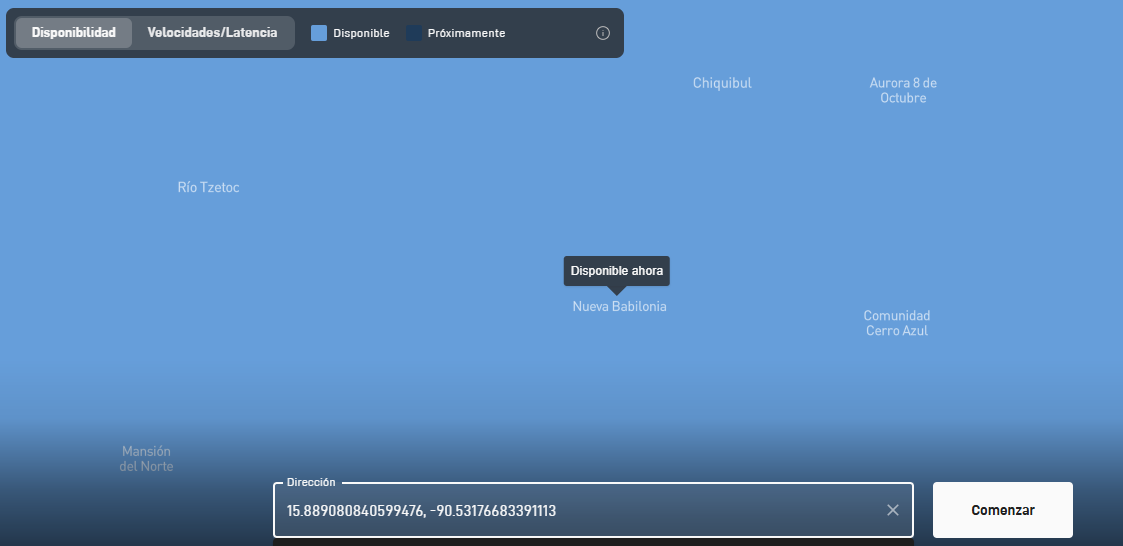
\includegraphics[width=.48\textwidth]{fig_ev_starlink_disponibilidad.png}\hfill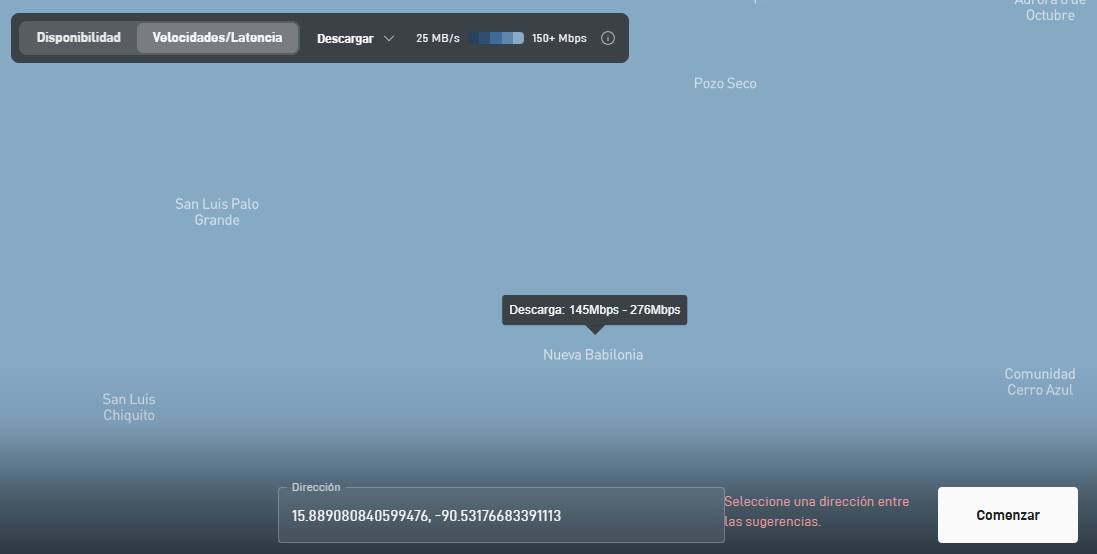
\includegraphics[width=.48\textwidth]{fig_ev_starlink_velocidades.png}\caption{Captura de starlink.com (23-oct-2026): servicio disponible en las coordenadas de la aldea y velocidades de 145 a 276\,Mbps de bajada \cite{F09}.}\label{fig:starlink}\end{figure}

\subsection{Aldea seleccionada}
Se eligi\'o la aldea \textbf{Babilonia} (el mapa de Starlink la rotula ``Nueva Babilonia''), municipio de Chisec, Alta Verapaz. Coordenadas del centro: $15.889081^\circ$\,N, $90.531767^\circ$\,O, elevaci\'on 206\,m s.\,n.\,m. No existe registro de censo a nivel de aldea; por ello, poblaci\'on y viviendas son \textbf{supuestos de dise\~no} declarados en la Secci\'on~\ref{sec:demanda}. La aldea mide aproximadamente 800\,m de largo y 270\,m de alto (16.7\,ha entre las esquinas aportadas).

\subsection{Objetivos y metas medibles}
\begin{enumerate}[nosep]
\item Conectar al menos el 95\,\% de las 109 edificaciones con enlace \'util (margen $\geq10$\,dB sobre el umbral del MCS elegido) en bajada y subida.
\item Ofrecer $\geq25$\,Mbps por punto en hora pico en el a\~no 3.
\item Autonom\'ia energ\'etica de al menos 2 d\'ias sin sol y disponibilidad objetivo $\geq99\,\%$.
\item CAPEX y OPEX calculados con fuentes y fecha, con costo por hogar.
\item Cumplir el marco regulatorio de la SIT, asumiendo que el proyecto lo ejecuta una empresa operadora ya legalizada.
\end{enumerate}
El proyecto lo realiza un equipo de tres personas (Kevin Gonz\'alez: arquitectura, enlace y simulaci\'on; Maximiliano Gonz\'alez: propagaci\'on, capacidad y energ\'ia; Diego Cuellar: costos, marco legal y presentaci\'on). La asignaci\'on completa de roles se detalla en la Secci\'on~\ref{sec:equipo}.

\section{La comunidad: geograf\'ia, terreno, vegetaci\'on y demanda}\label{sec:demanda}
\subsection{Viviendas y georreferenciaci\'on}
Sobre la imagen satelital se numeraron manualmente 109 edificaciones (Fig.~\ref{fig:casas}). Se advierte que la imagen puede estar desactualizada, que algunas casas pueden estar en construcci\'on o tapadas por \'arboles y que es dif\'icil distinguir una casa grande de dos contiguas; el an\'alisis toma las posiciones como correctas. Para pasar de p\'ixeles a metros se ajust\'o una transformaci\'on de similitud con 6 vectores torre--casa medidos en Google Earth: escala $0.514$\,m/p\'ixel, rotaci\'on $-0.07^\circ$ (norte arriba); residuos de 2--9\,m en las casas de control y $\approx\pm10$\,m en el resto.

\begin{figure}[H]\centering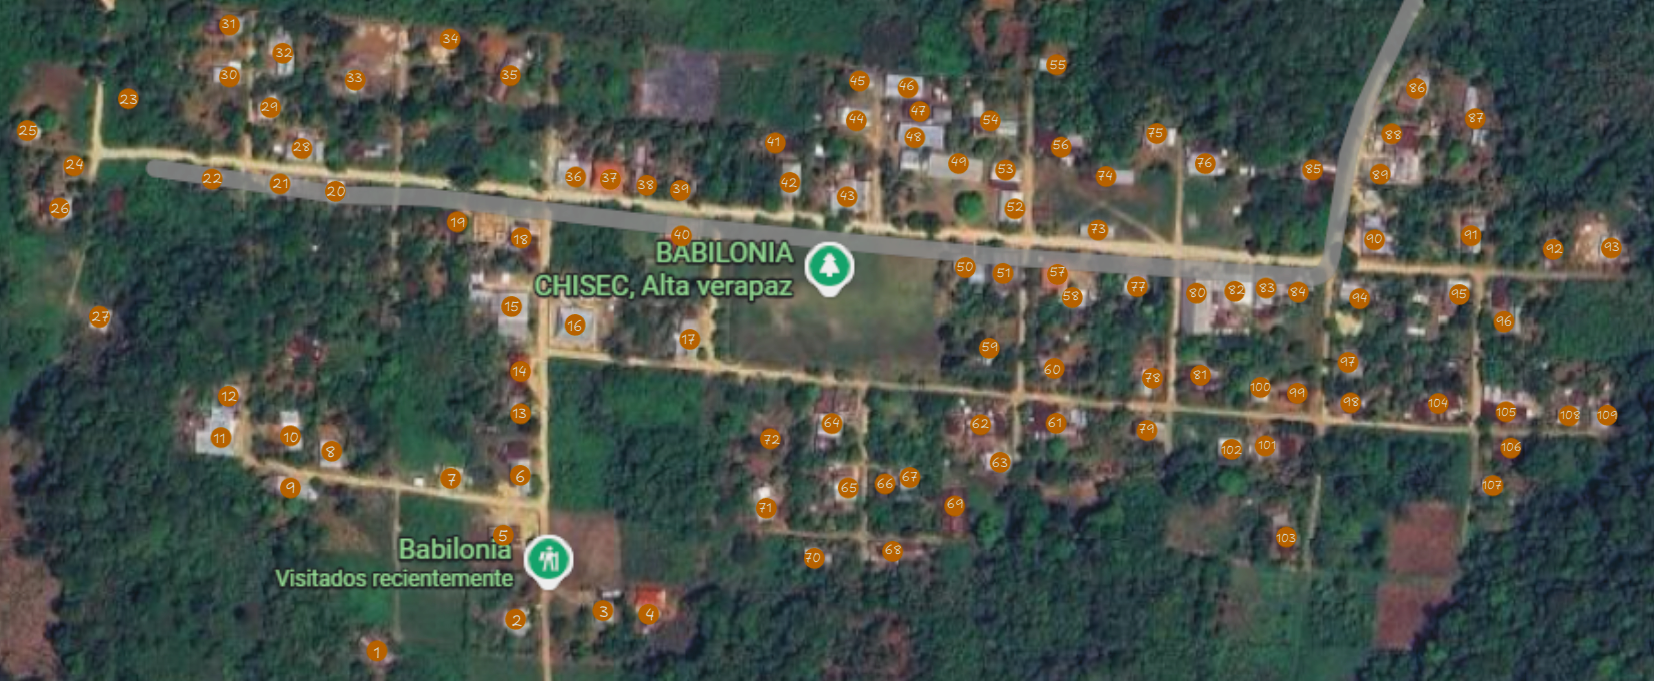
\includegraphics[width=.86\textwidth]{fig_ev_casas_numeradas.png}\caption{109 edificaciones numeradas sobre la imagen de Google Earth \cite{F13}.}\label{fig:casas}\end{figure}

La distancia horizontal a la torre central es m\'inima 50\,m, mediana 198\,m, percentil 90 de 354\,m y m\'axima 420\,m: 14 casas est\'an a $\leq$100\,m, 41 entre 100 y 200\,m, 28 entre 200 y 300\,m, 23 entre 300 y 400\,m y 3 a m\'as de 400\,m.

\subsection{Terreno}
Se midieron en Google Earth las elevaciones del centro (206\,m) y de las cuatro esquinas (215, 239, 247 y 227\,m) \cite{F12} y seis perfiles torre--casa (Fig.~\ref{fig:perf}) \cite{F15}. El terreno es una hondonada casi plana a 205--212\,m (oeste, norte, sur y centro) con una subida brusca en el extremo este hasta $\approx$237\,m; las casas 93 y 109 est\'an $\approx$30\,m por encima de la base de la torre. Con terreno desnudo, la l\'inea de vista desde una torre de $\geq3$\,m est\'a libre para las 109 casas: \textbf{el relieve no es el factor limitante}. El terreno se interpol\'o con funciones de base radial (\textit{thin-plate spline}) usando perfiles, esquinas y centro, con error $\leq1$\,m en las casas de control.

\begin{figure}[H]\centering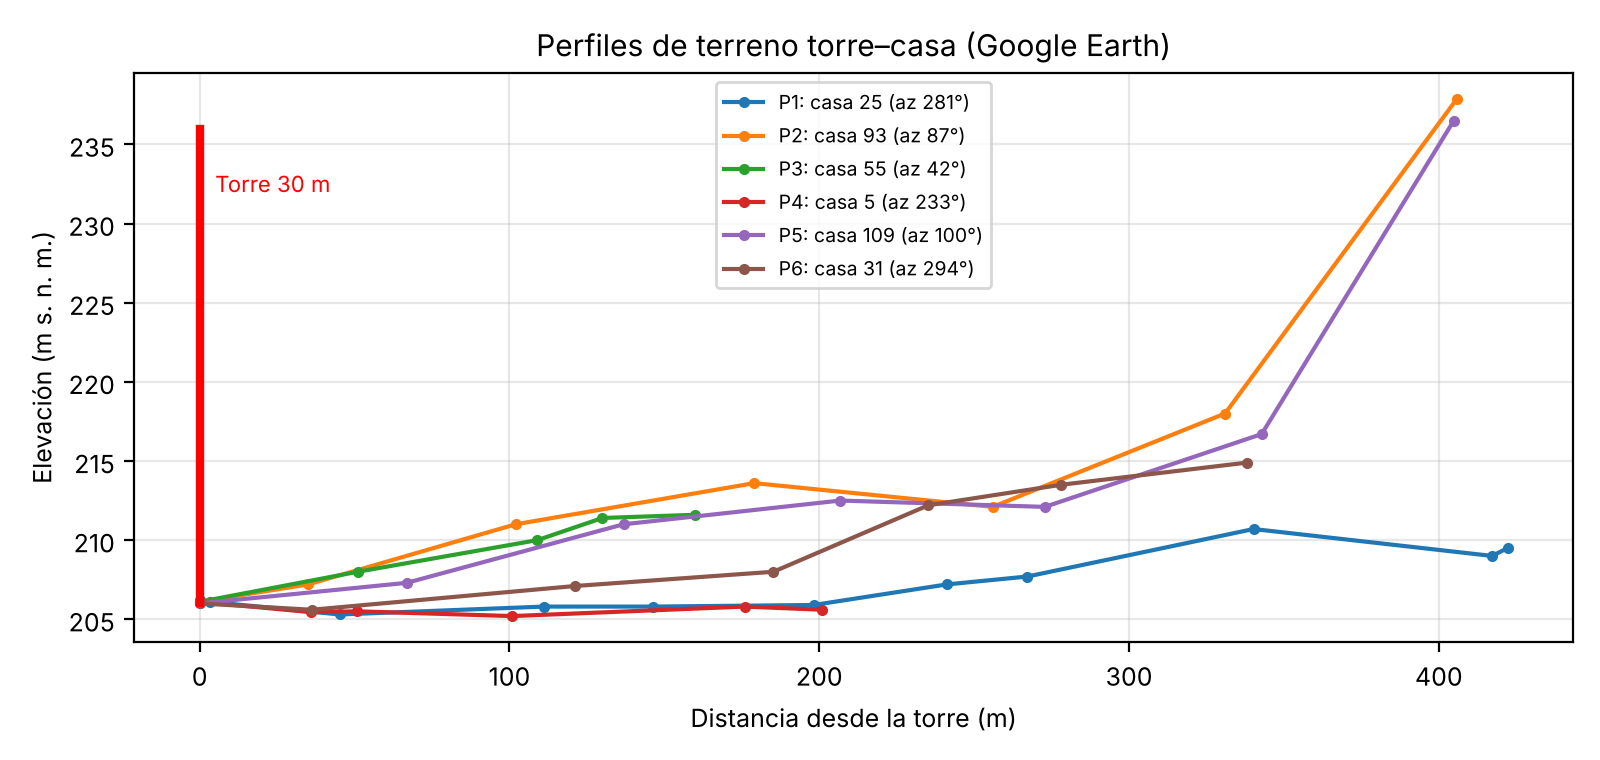
\includegraphics[width=.8\textwidth]{fig_perfiles_terreno.png}\caption{Perfiles de elevaci\'on torre--casa digitalizados de las capturas de Google Earth.}\label{fig:perf}\end{figure}

\subsection{Vegetaci\'on}
Con una m\'ascara por color (HSV) sobre la foto satelital se estim\'o que el 53\,\% de la imagen es copa de \'arbol. Se asume una altura de copa de 20\,m (sensibilidad 15 y 25\,m), y que los \'ultimos 10\,m del trayecto no cuentan, pues el CPE se monta en un m\'astil de 6\,m sobre el techo, en el lado m\'as despejado. La atenuaci\'on por follaje se calcula con el modelo de Weissberger \cite{F17}, con $f$ en GHz y $d$ la profundidad de follaje atravesada en metros:
\begin{equation}L_{fol}=\begin{cases}0.45\,f^{0.284}\,d & d\leq14\,\text{m}\\[2pt] 1.33\,f^{0.284}\,d^{0.588} & 14<d\leq400\,\text{m}\end{cases}\label{eq:weiss}\end{equation}
La Tabla~\ref{tab:follaje} y la Fig.~\ref{fig:follaje} muestran el efecto de la altura de torre; con 30\,m solo 4 casas superan 30\,dB (26, 27, 97 y 30). No se intenta ``despejar'' las copas (requerir\'ia m\'as de 100\,m de torre) sino presupuestar la p\'erdida.
\begin{table}[H]\centering\caption{P\'erdida por follaje (Weissberger, 5.8\,GHz) seg\'un altura de torre.}\label{tab:follaje}
\begin{tabular}{rrrrr}\toprule Torre (m) & Mediana (dB) & p90 (dB) & M\'axima (dB) & Casas $>$30\,dB\\\midrule 12 & 17.1 & 33.6 & 54.3 & 19\\ 18 & 17.1 & 33.6 & 54.3 & 18\\ 24 & 15.2 & 29.9 & 45.7 & 11\\ \textbf{30} & \textbf{12.0} & \textbf{27.4} & \textbf{41.2} & \textbf{4}\\ 36 & 10.8 & 24.8 & 37.8 & 2\\\bottomrule\end{tabular}\end{table}
\begin{figure}[H]\centering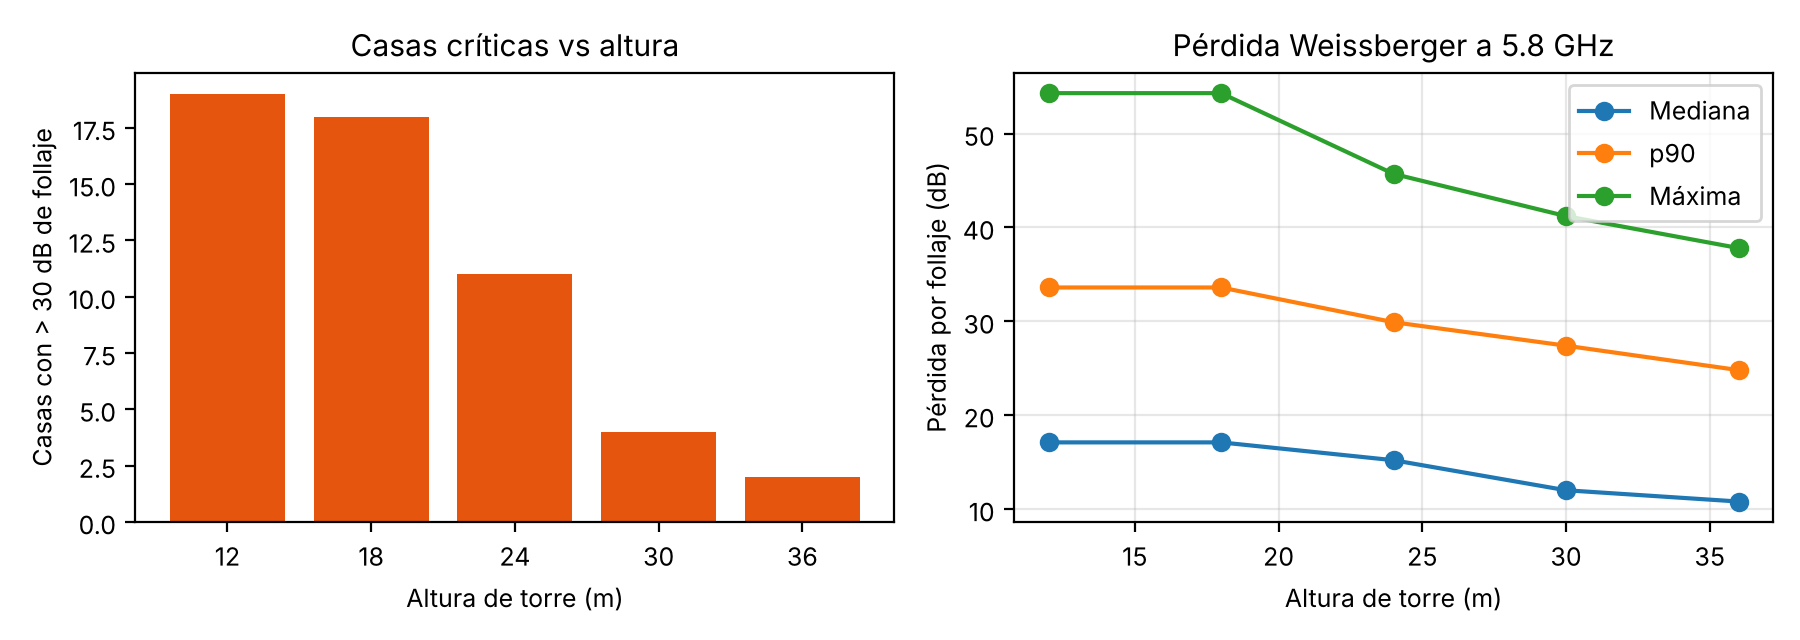
\includegraphics[width=.9\textwidth]{fig_follaje_vs_altura.png}\caption{Casas cr\'iticas y p\'erdida por follaje en funci\'on de la altura de la torre.}\label{fig:follaje}\end{figure}

\subsection{Poblaci\'on y modelo de demanda}
Las 109 edificaciones se consideran 95 viviendas habitadas ($\approx$87\,\%; el resto son tiendas, iglesia, bodegas o edificios secundarios), a 4.0 habitantes por vivienda (promedio nacional 4.5 \cite{F14}): $\approx$380 habitantes, 27\,\% sobre los $\approx$300 de referencia del enunciado, dentro de lo que el catedr\'atico admiti\'o. Si se exigiera 300, bastar\'ia 3.2 hab/vivienda sin cambiar el dise\~no, que se dimensiona por n\'umero de puntos de servicio (109) y no por habitantes.
\begin{table}[H]\centering\caption{Modelo de demanda.}\begin{tabular}{lrr}\toprule Par\'ametro & A\~no 1 & A\~no 3 (dise\~no)\\\midrule Puntos con CPE (adopci\'on 60\,\% / 90\,\%) & 65 & 98 + 2 hotspots\\ Consumo mensual por punto & 25\,GB & 25\,GB\\ Simultaneidad en hora pico & 25\,\% & 25\,\%\\ Tasa por usuario activo (DL/UL) & 4 / 0.5\,Mbps & 4 / 0.5\,Mbps\\ Pico agregado DL/UL & 65 / 8\,Mbps & 98 / 12\,Mbps\\ Uso del backhaul DL (145\,Mbps) & 45\,\% & 68\,\%\\\bottomrule\end{tabular}\end{table}
El backhaul se dise\~na con el l\'imite inferior medido en la zona (145\,Mbps de bajada, 21\,Mbps de subida, 32\,ms) \cite{F09,F11}.

\section{Alternativas de arquitectura}
Se compararon dos arquitecturas t\'ecnicamente distintas para la misma aldea.
\paragraph{A --- Torre central con acceso punto-multipunto (PtMP) en 5\,GHz.} Una torre ventada de 30\,m con el plato Starlink y tres radios con antenas sectoriales de 120\textdegree{}; una CPE direccional de 23\,dBi por casa. Un solo sitio con energ\'ia solar (Fig.~\ref{fig:sistema}).
\paragraph{B --- Malla Wi-Fi exterior multisalto.} 8 a 10 nodos en postes por la aldea, con un nodo pasarela conectado al Starlink (Fig.~\ref{fig:malla}); los usuarios se conectan por Wi-Fi 2.4/5\,GHz a su nodo m\'as cercano.
\begin{figure}[H]\centering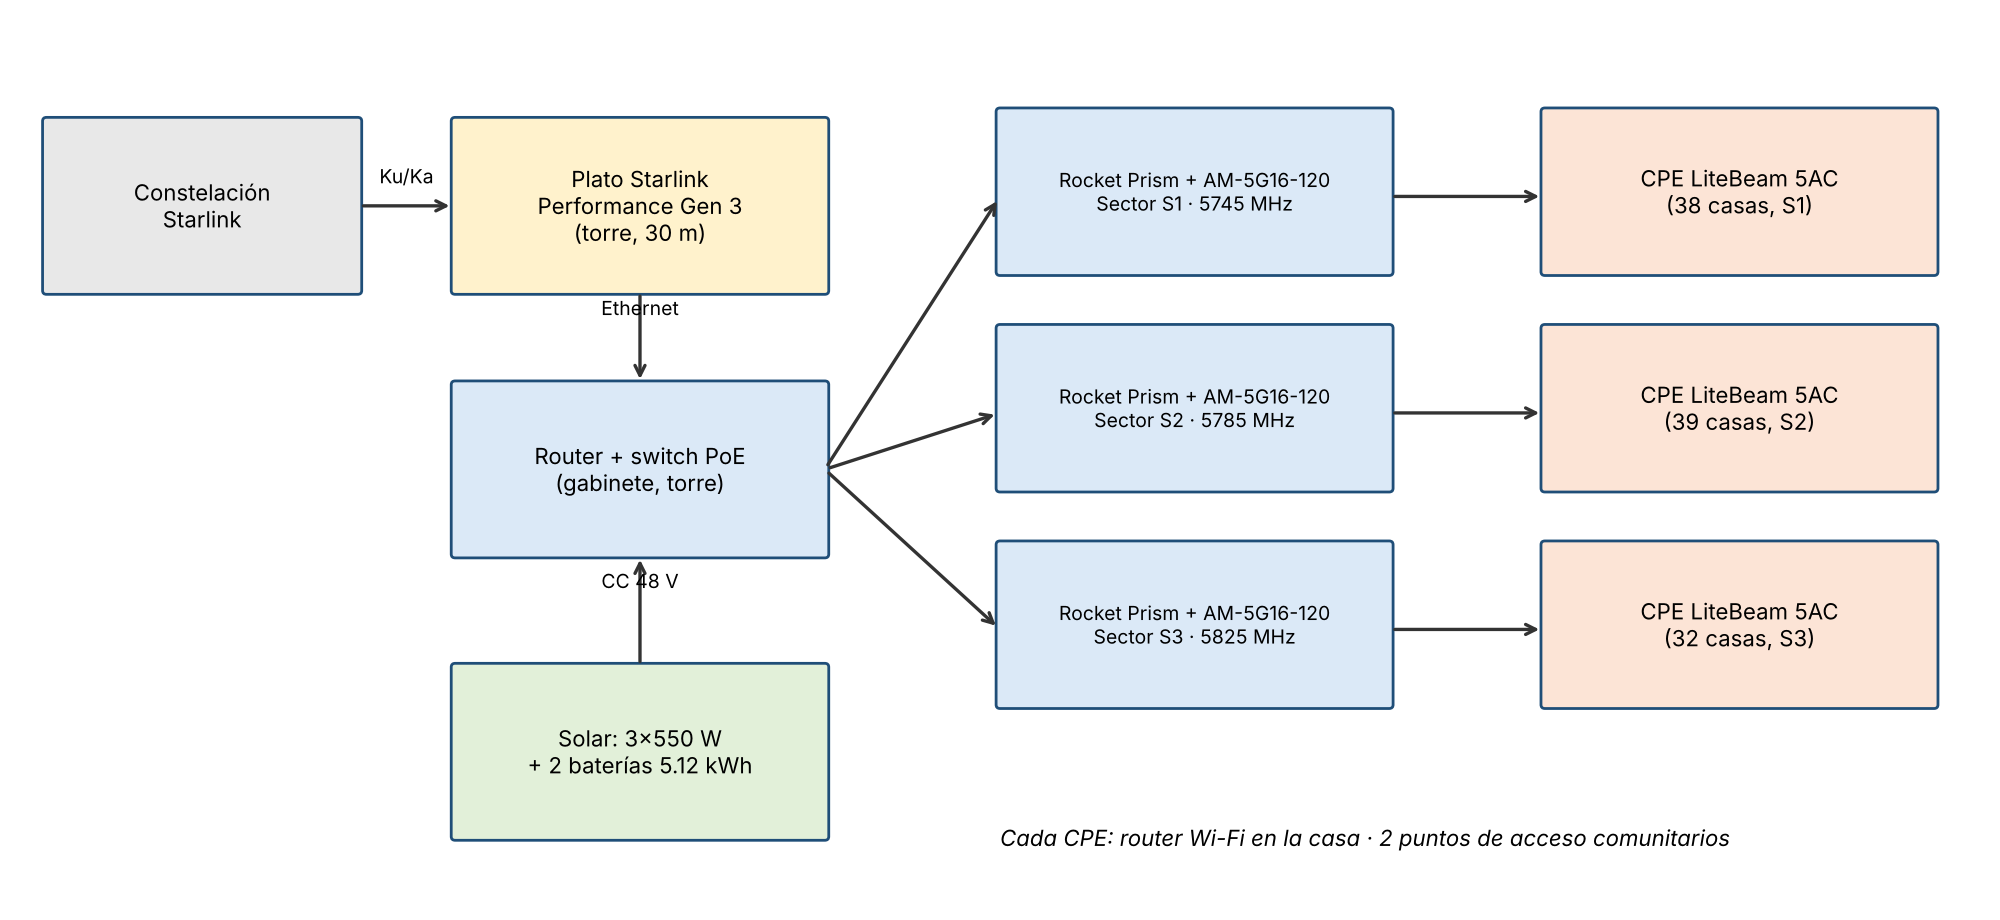
\includegraphics[width=\textwidth]{fig_diagrama_sistema.png}\caption{Diagrama de la arquitectura elegida (A).}\label{fig:sistema}\end{figure}
\begin{figure}[H]\centering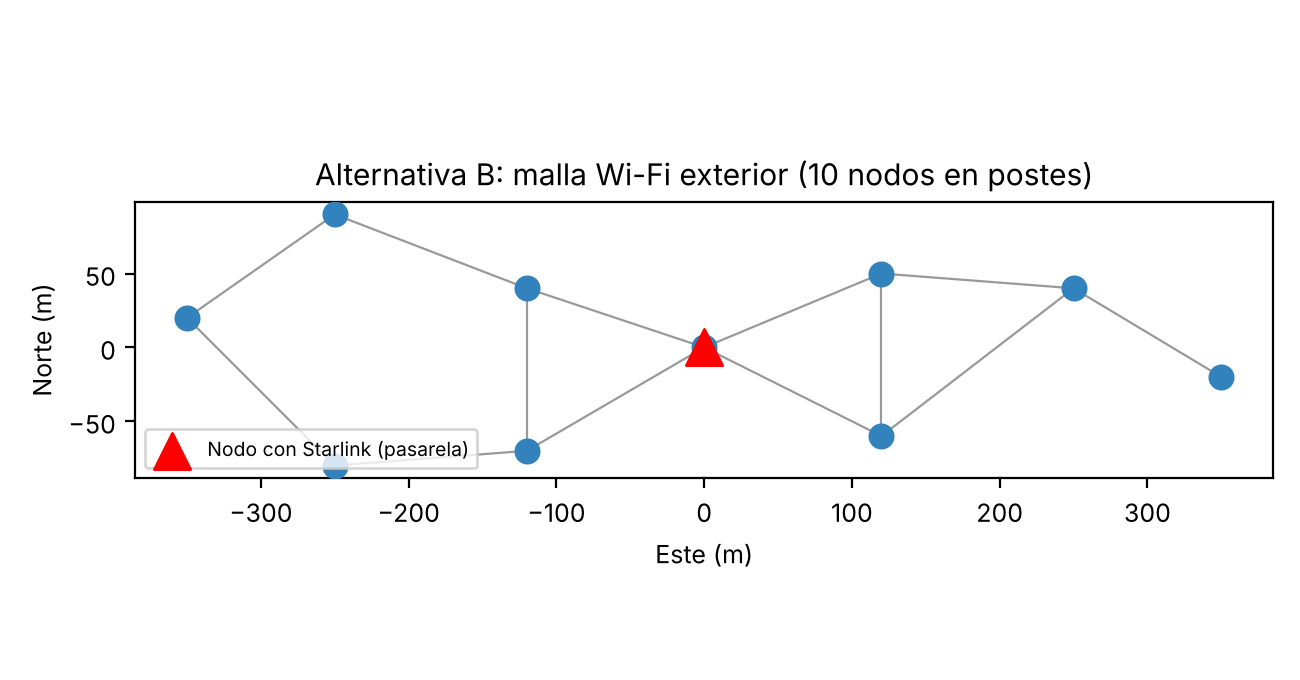
\includegraphics[width=.6\textwidth]{fig_arquitectura_B.png}\caption{Esquema de la alternativa B (malla).}\label{fig:malla}\end{figure}
\begin{table}[H]\centering\caption{Comparaci\'on de arquitecturas.}\label{tab:arq}\begin{tabular}{p{4cm}p{5.4cm}p{5.4cm}}\toprule & \textbf{A: torre central PtMP (elegida)} & \textbf{B: malla Wi-Fi}\\\midrule Sitios con energ\'ia solar & 1 & 8--10\\ Capacidad & Predecible, por sector con canal propio & Disminuye con cada salto (compartici\'on del medio)\\ Efecto del follaje & Un solo trayecto largo por casa, presupuestado & Trayectos cortos pero muchos puntos de falla\\ Latencia adicional & Un salto & 2--4 saltos\\ Mantenimiento & Un sitio alto + CPE & Muchos postes y bater\'ias\\ Costo relativo & Menor & Mayor (energ\'ia y mantenimiento por nodo)\\ Riesgo principal & Una sola torre (punto \'unico de falla) & Ca\'ida de capacidad y calidad\\\bottomrule\end{tabular}\end{table}
\textbf{Decisi\'on.} Se elige A por tener menos sitios con energ\'ia, capacidad predecible y un presupuesto de enlace verificable casa por casa. La \'unica torre es un punto \'unico de falla, mitigado con 2 d\'ias de autonom\'ia, equipo de repuesto y plan de crecimiento (Sec.~\ref{sec:cap}).

\section{Dise\~no del sistema de antenas}
\subsection{Inventario de antenas y radios}
\begin{table}[H]\centering\caption{Inventario de antenas del sistema. Datos de ficha salvo los marcados como supuesto o derivado.}\label{tab:inv}\small
\begin{tabular}{p{3.2cm}p{3.6cm}p{3.6cm}p{3.8cm}}\toprule Par\'ametro & Sectorial AM-5G16-120 (x3) & CPE LiteBeam 5AC Gen2 (x109) & Radio Rocket Prism 5AC Gen2 (x3)\\\midrule Banda & 5.10--5.85\,GHz & 5\,GHz (5150--5875) & 5150--5875\,MHz\\ Ganancia & 15--16\,dBi (15.5 usado) & 23\,dBi & Tx m\'ax. 28\,dBm\\ HPBW horizontal & 137\textdegree{} a 6\,dB (modelo: 97\textdegree{} a 3\,dB) & $\approx10^\circ$ (derivado de $70\lambda/D$) & ---\\ HPBW vertical & 8\textdegree{} (el\'ectrico) & $\approx10^\circ$ (derivado) & ---\\ Polarizaci\'on & Dual (V/H), aislamiento $\geq22$\,dB & Dual & MIMO 2x2\\ F/B & No indicado en ficha: tope supuesto 25\,dB & No indicado & ---\\ S11 / VSWR & VSWR $\leq1.5{:}1$ & --- & ---\\ Acimut / inclinaci\'on & 150\textdegree, 270\textdegree, 30\textdegree{} / 4\textdegree{} de f\'abrica + 0\textdegree{} & Hacia la torre / ---& ---\\ Altura & 30\,m en la torre & 6\,m sobre el techo & 29\,m (junto a la antena)\\ P\'erdida de cable/jumper & 0.5\,dB (supuesto) & Integrada & ---\\ Sensibilidad & --- & $-96$\,dBm (m\'ejor MCS) & $-96$ a $-65$\,dBm seg\'un MCS\\ Consumo & --- & 7\,W & 9.5\,W\\ Dimensiones/peso & 367x63x41\,mm, 1.1\,kg & 358x272x272\,mm, 0.98\,kg & 88x40x230\,mm, 0.4\,kg\\ Precio & US\$79 & US\$64.83 & US\$307.78\\\bottomrule\end{tabular}\end{table}
Fuentes: Rocket Prism \cite{F24}, AM-5G16-120 \cite{F25}, LiteBeam \cite{F27}. La alternativa AM-5G19-120 (18.6--19.1\,dBi, haz vertical 4\textdegree, 5.9\,kg) \cite{F26} se descart\'o: con 1--2\textdegree{} de inclinaci\'on mec\'anica logra margen m\'inimo similar (14--15\,dB) pero es sensible a errores de montaje de 1\textdegree, pierde 1--2 casas sin inclinaci\'on y pesa cinco veces m\'as sobre la torre.

\subsection{Relaci\'on con el principio f\'isico}
La sectorial es una apertura lineal en la dimensi\'on vertical (arreglo de elementos) con un reflector que forma el sector de 120\textdegree{} en horizontal. Para una apertura uniforme de longitud $L$, el ancho de haz a mitad de potencia es
\begin{equation}\mathrm{HPBW}\approx0.886\,\frac{\lambda}{L}\ \text{[rad]}\label{eq:hpbw}\end{equation}
A 5.8\,GHz, $\lambda=c/f=5.17$\,cm; con $L=0.367$\,m resulta $\mathrm{HPBW}=7.2^\circ$, en l\'inea con los 8\textdegree{} de la ficha. De la misma forma, la ganancia de una apertura crece con el \'area, $G=4\pi A\eta/\lambda^2$: la CPE (plato de $D=0.358$\,m, $\eta\approx0.55$--0.6) rinde $\approx23$\,dBi, y su haz $\approx70\lambda/D\approx10^\circ$ concentra la energ\'ia hacia la torre, lo que a la vez reduce la interferencia de otros sectores y de otras CPE. El haz vertical estrecho de la sectorial obliga a una inclinaci\'on hacia abajo ($4^\circ$ de f\'abrica): las casas cercanas quedan fuera del haz y se compensan con la menor distancia.

\subsection{Sectorizaci\'on y plan de frecuencias}
Los sectores se eligieron para equilibrar casas por sector (Fig.~\ref{fig:sect}): S1 (acimut 90--210\textdegree, eje 150\textdegree, 38 casas), S2 (210--330\textdegree, eje 270\textdegree, 39 casas) y S3 (330--90\textdegree, eje 30\textdegree, 32 casas).
\begin{table}[H]\centering\caption{Plan de frecuencias, una portadora por sector.}\begin{tabular}{lrrrll}\toprule Sector & Eje & Canal central & Ancho & Polarizaci\'on & Sincron\'ia\\\midrule S1 & 150\textdegree & 5745\,MHz & 20\,MHz & H/V (MIMO 2x2) & GPS\\ S2 & 270\textdegree & 5785\,MHz & 20\,MHz & H/V & GPS\\ S3 & 30\textdegree & 5825\,MHz & 20\,MHz & H/V & GPS\\\bottomrule\end{tabular}\end{table}
Los tres canales caen dentro de 5725--5850\,MHz, que figura entre las bandas de 5\,GHz de Guatemala \cite{F28} (Sec.~\ref{sec:legal}). La sincron\'ia GPS entre los tres radios alinea las tramas TDD y evita interferencia entre bajada y subida de sectores vecinos.
\begin{figure}[H]\centering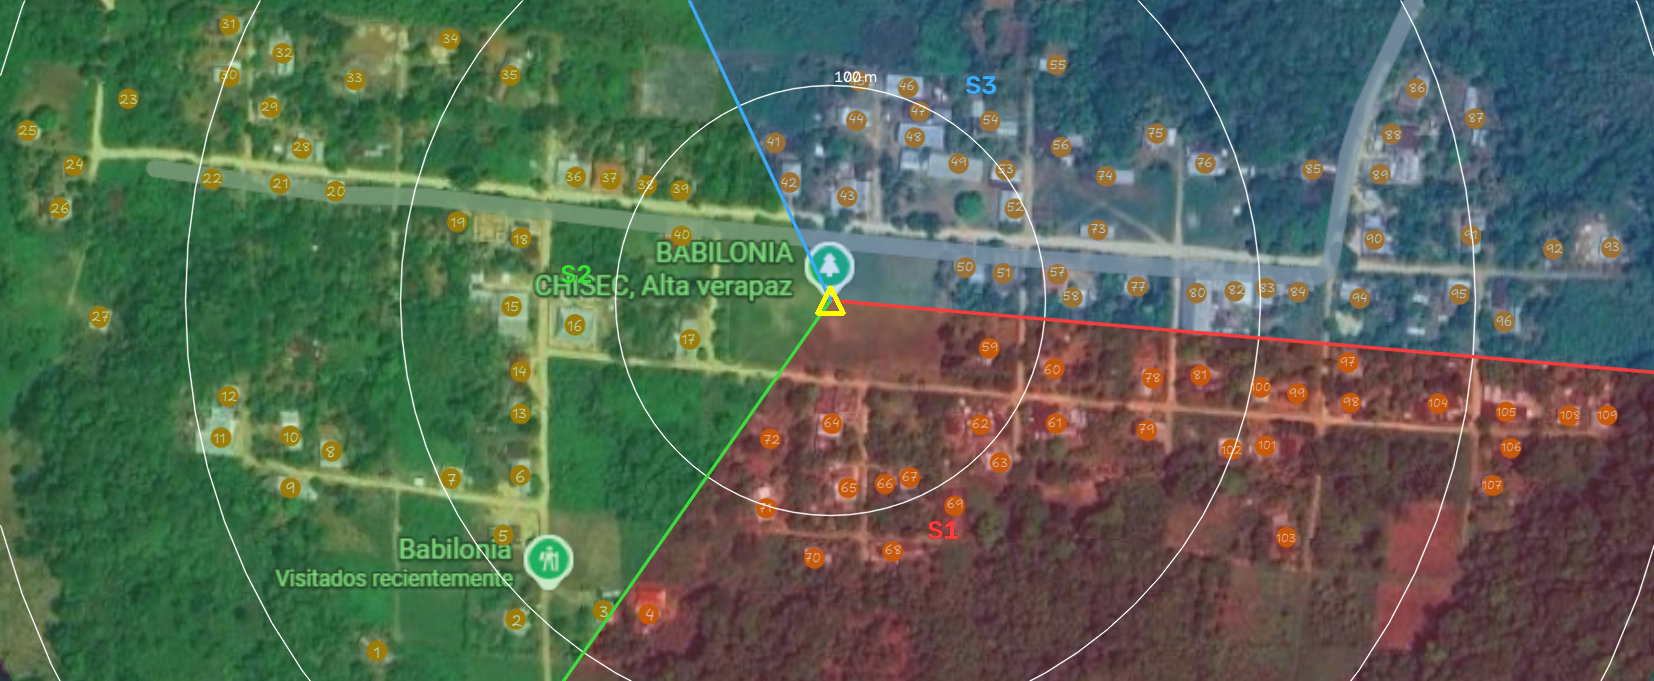
\includegraphics[width=.85\textwidth]{fig_aldea_sectores_prelim.png}\caption{Casas, torre y sectores (acimut respecto al norte).}\label{fig:sect}\end{figure}

\section{Patrones de radiaci\'on}
La Fig.~\ref{fig:patron} muestra los cortes horizontal y vertical de la sectorial AM-5G16-120. Las referencias de la ficha son: ganancia 15--16\,dBi, ancho de haz horizontal 137\textdegree{} a 6\,dB, elevaci\'on 8\textdegree{} \cite{F25}. \textbf{Declaraci\'on de origen:} los cortes son un \textbf{modelo} calibrado con esos valores de ficha (no son patrones medidos): en acimut, una par\'abola en dB que pasa por $-6$\,dB a $\pm68.5^\circ$ (los puntos rojos son datos de ficha) con piso de 25\,dB; en elevaci\'on, el patr\'on de una apertura uniforme de 0.367\,m, $|\sin u/u|$ con $u=\pi (L/\lambda)\sin\theta$, que da un haz de 7.0\textdegree{} a 3\,dB, primer nulo en $\pm8.5^\circ$ y primeros lóbulos laterales a $-13$\,dB. La ficha no publica F/B ni lóbulos laterales; se supone un tope de 25\,dB y se verifica su efecto en la interferencia (Sec.~\ref{sec:interf}).
\begin{figure}[H]\centering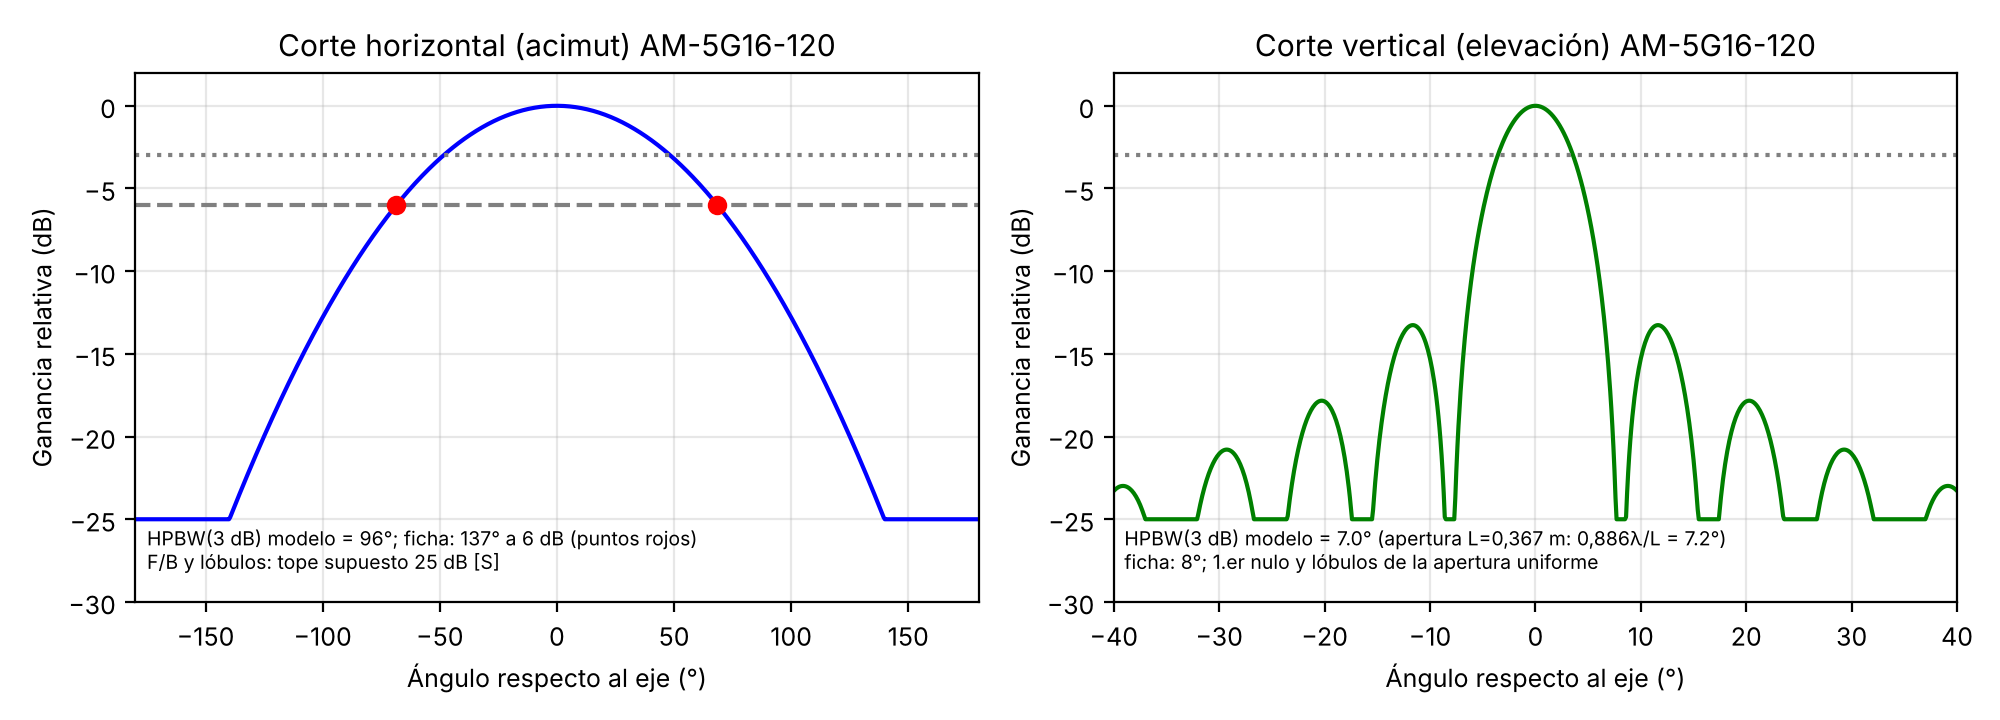
\includegraphics[width=\textwidth]{fig_patron_sectorial_H_V.png}\caption{Cortes H y V de la sectorial (modelo calibrado con ficha).}\label{fig:patron}\end{figure}
\begin{figure}[H]\centering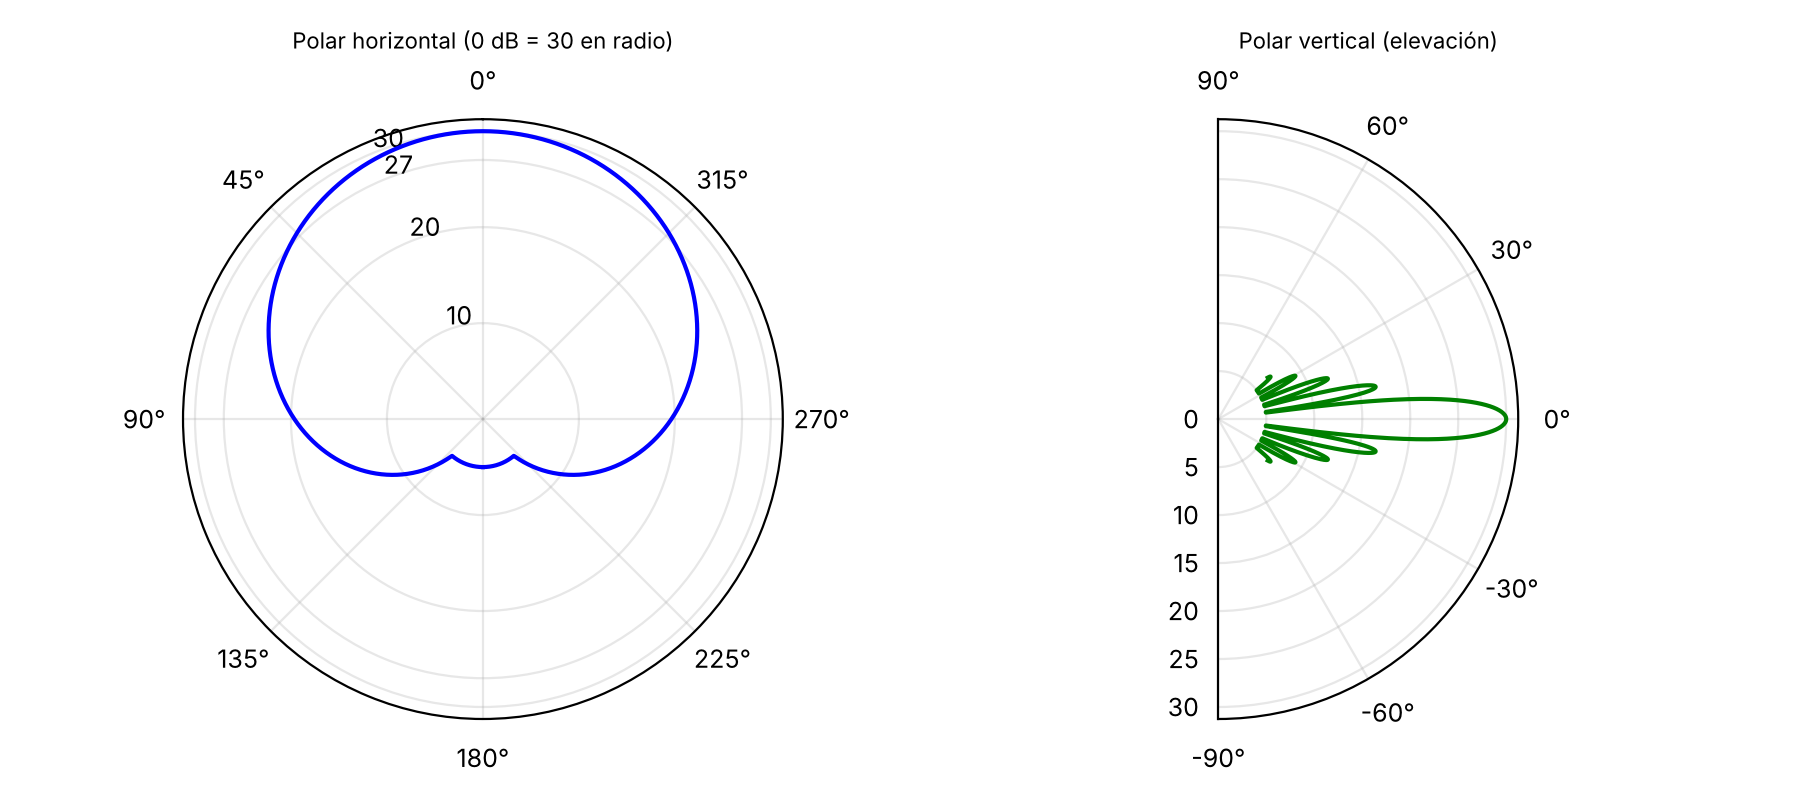
\includegraphics[width=.8\textwidth]{fig_patron_sectorial_polar.png}\caption{Patrones en coordenadas polares.}\end{figure}

\section{Propagaci\'on}
\subsection{P\'erdida en espacio libre}
\begin{equation}\mathrm{FSPL}=32.44+20\log_{10}d_{\mathrm{km}}+20\log_{10}f_{\mathrm{MHz}}\label{eq:fspl}\end{equation}
A 5.8\,GHz: 82.4\,dB a 50\,m y 99.9\,dB a 420\,m.
\subsection{Zona de Fresnel y despeje}
El radio de la primera zona de Fresnel es $r_1=\sqrt{\lambda d_1d_2/(d_1+d_2)}$; en el punto medio del enlace m\'as largo (420\,m) vale $r_1=\sqrt{0.0517\cdot210\cdot210/420}\approx2.3$\,m (60\,\% $\approx1.4$\,m). Con el terreno desnudo, la altura m\'inima de torre por casa que despeja el 60\,\% de $r_1$ es $\leq2.8$\,m para las 109 casas (\texttt{los\_altura\_minima\_por\_casa.csv}); la torre de 30\,m supera con amplio margen el despeje geom\'etrico, incluso para el extremo este elevado.
\subsection{Difracci\'on}
Como el perfil no presenta obst\'aculos de relieve sobre la l\'inea de vista, la difracci\'on por filo de cuchillo no aporta p\'erdida de dise\~no; la \'unica obstrucci\'on es la vegetaci\'on, tratada como medio absorbente (Weissberger). Para las dos casas del extremo este, a $\approx$30\,m sobre la base de la torre, el rayo baja ligeramente y sigue libre del relieve (aunque cruza algo de follaje).
\subsection{Vegetaci\'on}
Ver Ec.~\eqref{eq:weiss}. Con 30\,m de torre y copas de 20\,m, la p\'erdida por follaje tiene mediana de 12.0\,dB, percentil 90 de 27.4\,dB y m\'aximo de 41.2\,dB (casa 26).
\subsection{Lluvia y otros}
La lluvia a 5.8\,GHz sobre trayectos $\leq0.42$\,km aporta menos de 0.3\,dB seg\'un el orden de magnitud de UIT-R P.838-3 (valor por verificar en la Recomendaci\'on); se incluye 0.3\,dB y un escenario de desvanecimiento extra de 6\,dB (Sec.~\ref{sec:sens}).

\section{Presupuesto de enlace}
\subsection{M\'etodo}
Para cada casa se calcula, en bajada (AP$\to$CPE) y subida (CPE$\to$AP), la potencia recibida
\begin{equation}P_r=P_t+G_{AP}^{ef}-L_{feed}+G_{CPE}-\mathrm{FSPL}-L_{fol}-L_{mis}-L_{lluvia}\end{equation}
con $G_{AP}^{ef}=G_{AP}-L_{az}(\Delta\mathrm{az})-L_{el}(\Delta\mathrm{el})$, donde $\Delta$az es el desfase respecto al eje del sector y $\Delta$el la diferencia entre el \'angulo de elevaci\'on del rayo y la inclinaci\'on de la antena. El margen es $M=P_r-(S_{MCS}+3\,\mathrm{dB})$, donde $S_{MCS}$ es la sensibilidad de ficha del radio \cite{F24} y 3\,dB es una penalizaci\'on conservadora por usar canal de 20\,MHz. Se elige el mayor MCS cuyo margen sea $\geq10$\,dB, cada uno con su propia potencia de transmisi\'on m\'axima (28 a 22\,dBm). En subida la CPE transmite 3\,dB menos (25 frente a 28\,dBm). La tasa PHY es $2\cdot52\cdot b\cdot r_c/3.6\,\mu$s (canal de 20\,MHz, 2x2).
\begin{table}[H]\centering\caption{Par\'ametros del presupuesto de enlace.}\small\begin{tabular}{llr}\toprule Par\'ametro & Valor & Origen\\\midrule Frecuencia & 5.8\,GHz & Dise\~no\\ Potencia Tx AP / CPE & 28 / 25\,dBm & Ficha \cite{F24,F27}\\ Ganancia AP / CPE & 15.5 / 23\,dBi & Ficha \cite{F25,F27}\\ Jumpers $L_{feed}$ & 0.5\,dB & Supuesto\\ Desalineaci\'on CPE & 1.0\,dB & Supuesto\\ Lluvia & 0.3\,dB & UIT-R P.838-3 (aprox.)\\ Penalizaci\'on 20\,MHz & 3\,dB & Supuesto conservador\\ Margen de dise\~no & 10\,dB & Criterio del proyecto\\ Eficiencia MAC / DL de la trama & 0.65 / 0.75 & Supuesto\\\bottomrule\end{tabular}\end{table}
\subsection{Ejemplo detallado: casa 26 (peor caso, sector S2, subida)}
Distancia horizontal 398.1\,m; desnivel antena--CPE 29.0\,m $\Rightarrow$ distancia 3D 398.6\,m, elevaci\'on del rayo $2.8^\circ$ ($\Delta$el $=-1.2^\circ$ respecto a los $4^\circ$ de inclinaci\'on); $\Delta$az $=6.2^\circ$. Entonces $L_{az}=6(2\cdot6.2/137)^2=0.05$\,dB y $L_{el}\approx0.4$\,dB, y $G_{AP}^{ef}=15.1$\,dBi. FSPL $=32.44+20\log_{10}0.3986+20\log_{10}5800=99.7$\,dB. Follaje: profundidad 147\,m $\Rightarrow$ $L_{fol}=1.33\cdot5.8^{0.284}\cdot147^{0.588}=41.2$\,dB. En subida, con BPSK 1/2 y $P_t=25$\,dBm:
\[P_r=25+23-0.5+15.1-99.7-41.2-1.0-0.3=-79.6\,\mathrm{dBm},\quad M=-79.6-(-96+3)=13.4\,\mathrm{dB}\]
que cumple $\geq10$\,dB (MCS \'util en subida: QPSK 1/2; en bajada, 16QAM 1/2 con 16.4\,dB sobre BPSK).
\subsection{Resultados}
\begin{table}[H]\centering\caption{Presupuesto de enlace por rango de distancia (DL = bajada, UL = subida).}\small\resizebox{\textwidth}{!}{\begin{tabular}{lrrrrrrl}\toprule Rango (m) & Casas & $G_{AP}$ efec. (dBi) & FSPL (dB) & Follaje (dB) & Margen DL med. (dB) & Margen UL mín. (dB) & MCS DL más común\\\midrule
0--100 & 14 & -2.1 & 86.3 & 0.0 & 50.7 & 39.0 & 256QAM 5/6\\
100--200 & 41 & 8.9 & 90.6 & 8.2 & 49.7 & 22.8 & 256QAM 5/6\\
200--300 & 28 & 12.9 & 96.0 & 16.9 & 42.1 & 23.6 & 64QAM 5/6\\
300--400 & 23 & 12.2 & 98.3 & 21.6 & 34.6 & 13.4 & 64QAM 5/6\\
400--500 & 3 & 6.2 & 99.9 & 9.6 & 46.7 & 34.8 & 256QAM 3/4\\\bottomrule\end{tabular}
}\end{table}
\begin{table}[H]\centering\caption{Peor caso por sector y casos tipo.}\small\resizebox{\textwidth}{!}{\begin{tabular}{lrrrrrrrrrr}\toprule Caso & Casa & Dist. (m) & $\Delta$az (°) & $\Delta$el (°) & $G_{AP}$ ef. & FSPL & Follaje & Margen DL & Margen UL & MCS DL \\\midrule
Peor S1 & 107 & 355 & -43.7 & -3.5 & 10.2 & 98.7 & 28.4 & 25.3 & 22.3 & 64QAM 2/3\\
Peor S2 & 26 & 398 & 6.2 & -1.2 & 15.1 & 99.7 & 41.2 & 16.4 & 13.4 & 16QAM 1/2\\
Peor S3 & 86 & 319 & 40.9 & -2.7 & 11.7 & 97.8 & 27.7 & 28.3 & 25.3 & 64QAM 2/3\\
Casa más cercana & 43 & 50 & -19.5 & 20.4 & -2.8 & 82.4 & 0.0 & 57.0 & 54.0 & 256QAM 5/6\\
Casa mediana & 35 & 198 & 34.1 & 1.5 & 13.5 & 93.7 & 6.7 & 55.4 & 52.4 & 256QAM 5/6\\
\bottomrule\end{tabular}
}\end{table}
\begin{table}[H]\centering\caption{Resumen por sector.}\small\resizebox{\textwidth}{!}{\begin{tabular}{lrrrrrr}\toprule Sector & Casas & Dist. máx. (m) & Follaje mediano (dB) & Margen mín. DL (dB) & Margen mín. UL (dB) & Util. aire DL/UL\\\midrule
S1 & 38 & 405 & 12.0 & 25.3 & 22.3 & 44\,\% / 18\,\%\\
S2 & 39 & 420 & 18.9 & 16.4 & 13.4 & 48\,\% / 21\,\%\\
S3 & 32 & 402 & 4.8 & 28.3 & 25.3 & 34\,\% / 13\,\%\\\bottomrule\end{tabular}
}\end{table}
\begin{figure}[H]\centering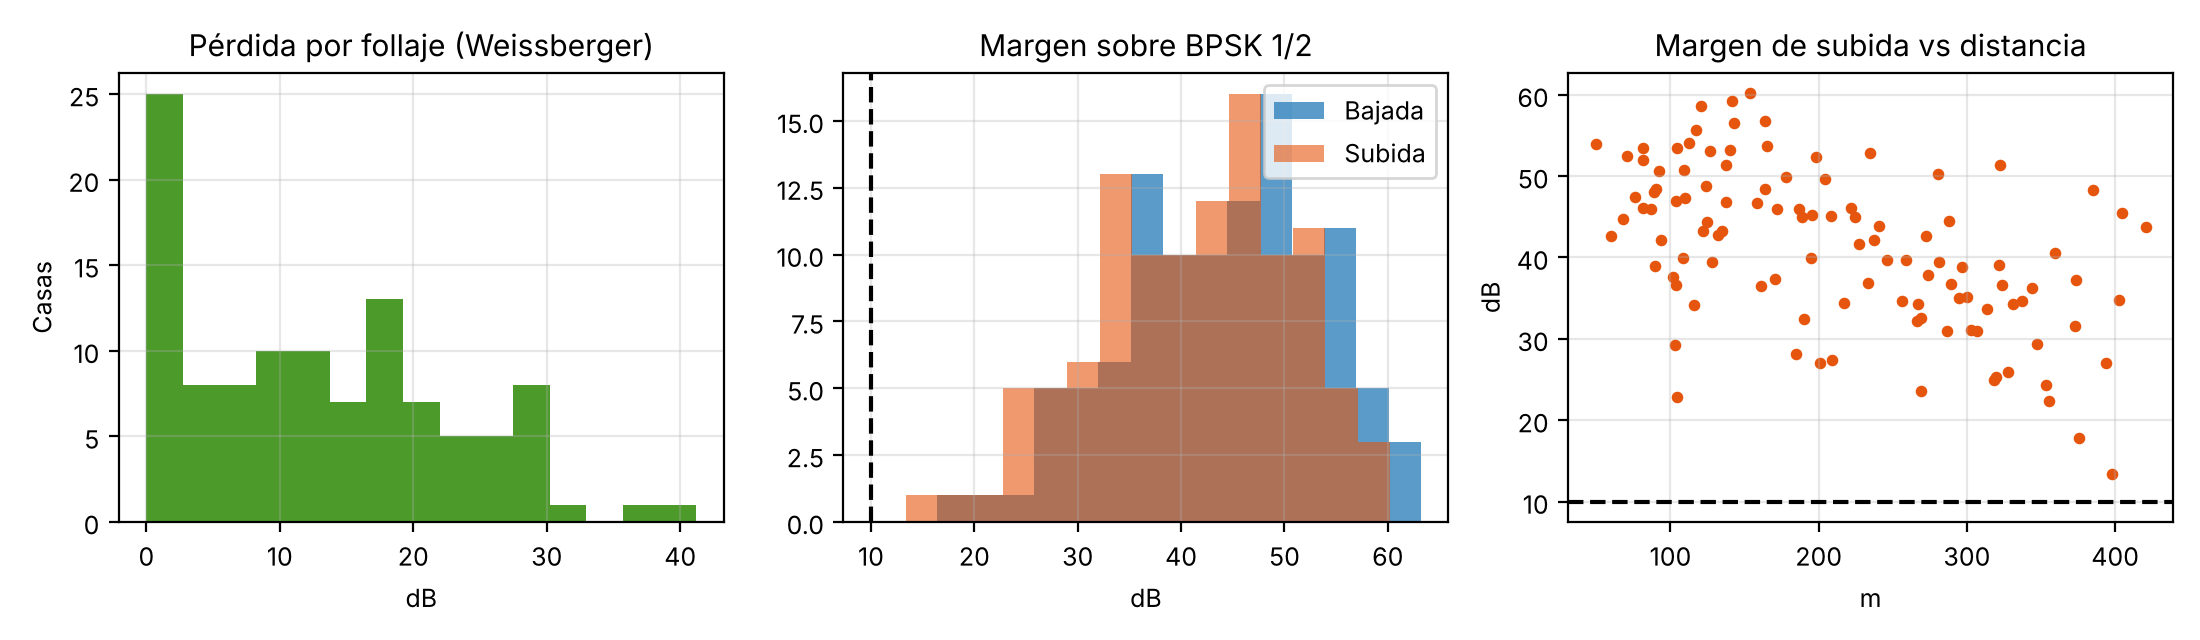
\includegraphics[width=\textwidth]{fig_histogramas_enlace.png}\caption{Distribuci\'on de p\'erdida por follaje, m\'argenes de enlace y margen de subida frente a distancia.}\end{figure}
Resultado: \textbf{109 de 109 casas} tienen MCS \'util en bajada y subida con margen $\geq10$\,dB. En bajada, 47 casas alcanzan 256QAM 5/6 y 20 casas 256QAM 3/4; 40 usan 64QAM y 2 usan 16QAM (Tabla~\ref{tab:mcs}). Las 14 casas a $\leq100$\,m caen en los l\'obulos de elevaci\'on de la sectorial ($G_{AP}^{ef}$ mediana $-2.1$\,dBi) pero su corta distancia mantiene m\'argenes de 39\,dB o m\'as en subida.
\begin{table}[H]\centering\caption{MCS m\'aximo usable en bajada.}\label{tab:mcs}\begin{tabular}{lr}\toprule MCS (bajada, DL) & Casas\\\midrule
256QAM 5/6 & 47\\
256QAM 3/4 & 20\\
64QAM 5/6 & 27\\
64QAM 3/4 & 5\\
64QAM 2/3 & 8\\
16QAM 3/4 & 1\\
16QAM 1/2 & 1\\\bottomrule\end{tabular}
\end{table}
\textbf{Contingencia (regla de dise\~no D08).} Si m\'as de 6 casas ($\approx$5\,\%) quedaran con margen $<10$\,dB, se aplicar\'ia, en orden: CPE de mayor ganancia o m\'astil de 10\,m en esas casas; nodo de relevo en la zona alta del este; m\'as altura de torre. Con el dise\~no base no se activa.

\section{Cobertura, interferencia y sectores}\label{sec:interf}
La Fig.~\ref{fig:cob} muestra el MCS m\'aximo por casa. Para la interferencia entre sectores se calcul\'o, para cada casa, la potencia del sector propio y de los dos vecinos usando el mismo modelo de patrones, con ruido de $-95$\,dBm (20\,MHz, figura de ruido 6\,dB) y rechazo de canal adyacente de 30\,dB. Con un solo canal para los tres sectores, la relaci\'on portadora/interferencia (C/I) cocanal tiene m\'inimo 0\,dB, mediana 8\,dB y percentil 10 de 1\,dB: 40 casas quedar\'ian sin MCS usable y la utilizaci\'on del aire llegar\'ia a 144\,\% en S2. Con tres canales separados, ninguna casa queda sin enlace y la utilizaci\'on m\'axima baja a 48\,\%. Esto justifica el plan de frecuencias de tres canales con sincron\'ia GPS.
\begin{figure}[H]\centering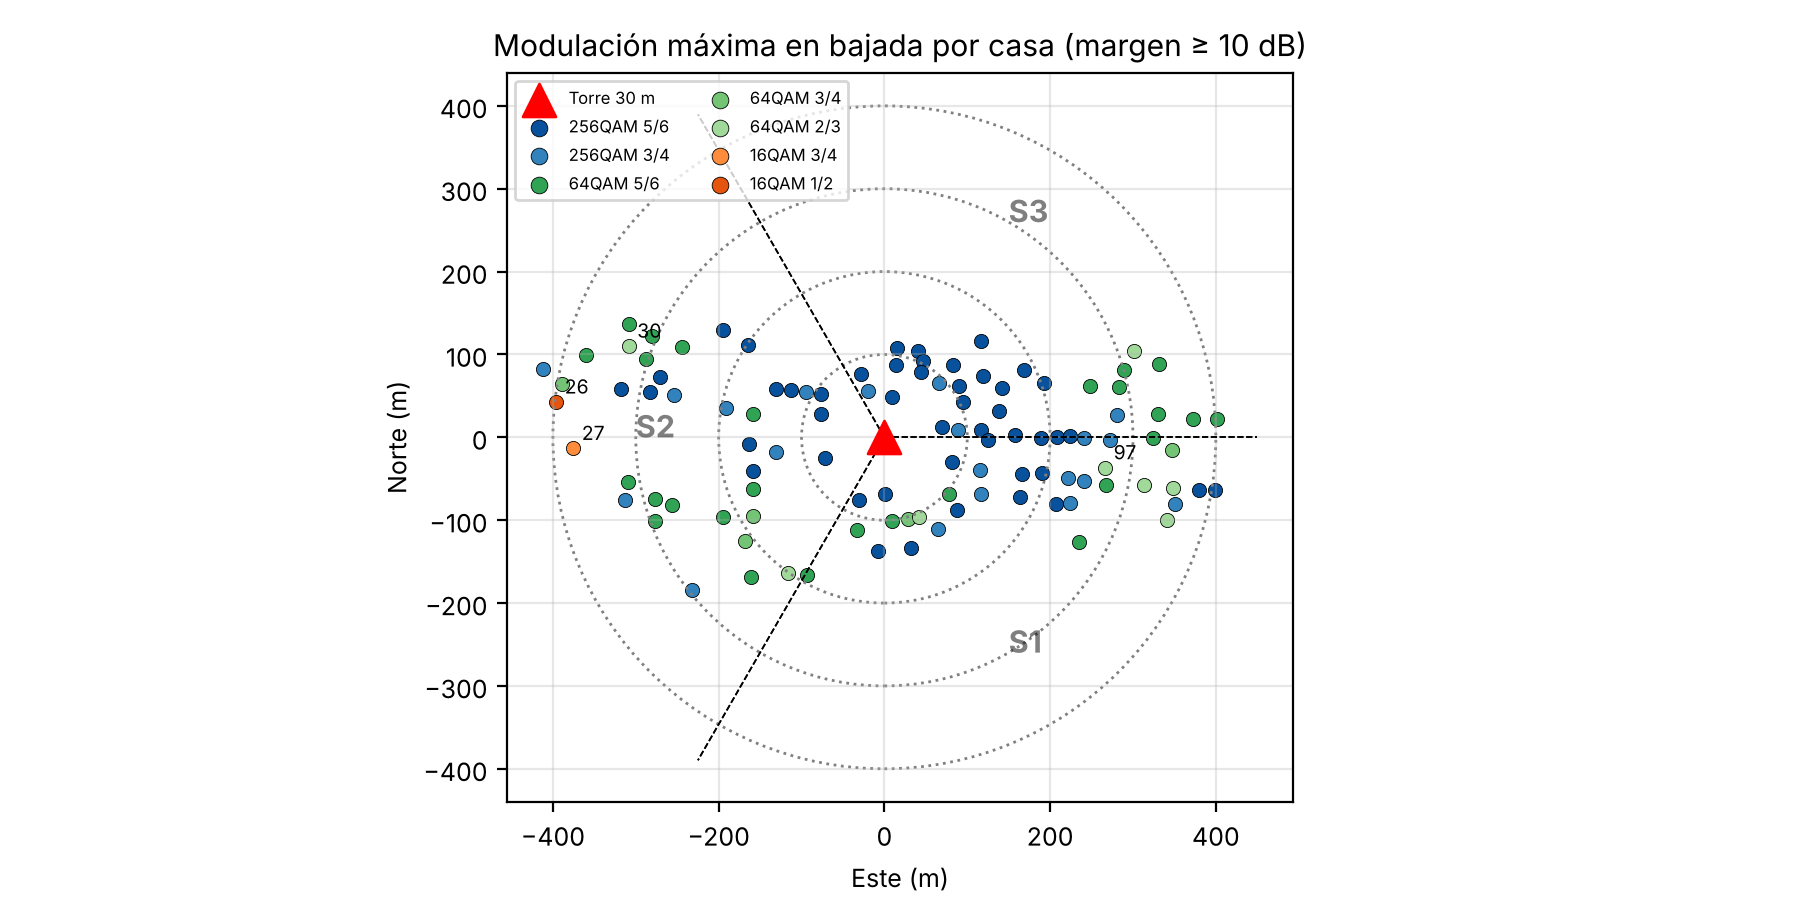
\includegraphics[width=.92\textwidth]{fig_cobertura_mcs.png}\caption{Modulaci\'on m\'axima en bajada por casa (margen $\geq10$\,dB), torre y l\'imites de sector.}\label{fig:cob}\end{figure}

\section{Capacidad}\label{sec:cap}
La utilizaci\'on de aire de un sector es $U=\frac{1}{\text{fracci\'on DL}}\sum_i \frac{a\,\rho}{\eta\,R_i}$, donde $a$ es la adopci\'on, $\rho$ la demanda media por suscriptor (1\,Mbps en bajada y 0.125\,Mbps en subida: 4\,Mbps y 0.5\,Mbps por 25\,\% de simultaneidad), $\eta=0.65$ la eficiencia MAC y $R_i$ la tasa PHY de cada casa (equidad de tiempo de aire). Resultados del a\~no 3 (90\,\%): S1 44\,\%, S2 48\,\%, S3 34\,\% en bajada, y 18, 21 y 13\,\% en subida; el backhaul Starlink se usa al 68\,\% en bajada y 58\,\% en subida. Escenarios de crecimiento (utilizaci\'on DL S1/S2/S3): a\~no 1 $29/32/23\,\%$; a\~no 5 con 100\,\% de adopci\'on y 6\,Mbps de pico $73/81/57\,\%$; con 8\,Mbps $97/107/76\,\%$, caso en el que S2 se saturar\'ia y habr\'ia que a\~nadir un cuarto sector o un segundo radio por sector. El segundo terminal Starlink se planifica para la fase 2 si el uso pico supera 70\,\%.

\section{Simulaci\'on, sensibilidad y validaci\'on}\label{sec:sens}
\subsection{Herramientas y verificaci\'on cruzada}
El modelo se implement\'o dos veces: en Python (\texttt{linkbudget.py}) y en Excel con f\'ormulas visibles (hoja \texttt{Enlace\_por\_casa}); ambos coinciden en las 109 casas (diferencia m\'axima de margen 0.14\,dB, debida al redondeo de entradas). Para contrastar un c\'alculo con una herramienta de RF independiente se simulan en CloudRF cuatro enlaces (casas 26, 43, 55 y 93) con los par\'ametros de la Tabla~\ref{tab:cloudrf}.
\begin{table}[H]\centering\caption{Contraste con simulador RF (CloudRF). Columnas del simulador a completar con la captura.}\label{tab:cloudrf}\small\begin{tabular}{rrrrrr}\toprule Casa & Dist. (m) & FSPL propio (dB) & Pr propia (dBm) & Pr CloudRF (dBm) & Diferencia\\\midrule 26 & 398 & 99.7 & $-76.6$ & por simular & ---\\ 43 & 50 & 82.4 & $-36.0$ & por simular & ---\\ 55 & 165 & 92.1 & $-36.3$ & por simular & ---\\ 93 & 402 & 99.8 & $-55.2$ & por simular & ---\\\bottomrule\end{tabular}\end{table}
\subsection{Sensibilidad}
Se recalcul\'o todo el modelo para escenarios de altura de torre, altura de copa, desvanecimiento adicional y error de montaje (Tabla~\ref{tab:sens}, Fig.~\ref{fig:sens}).
\begin{table}[H]\centering\caption{Escenarios de sensibilidad.}\label{tab:sens}\small\begin{tabular}{p{6.4cm}rrrr}\toprule Escenario & Casas útiles & Margen DL mín. & Margen UL mín. & Casas $>$30 dB\\\midrule
Base: torre 30 m, copa 20 m & 109 & 16.4 & 13.4 & 4\\
Torre 24 m & 108 & 11.3 & 8.3 & 11\\
Torre 36 m & 109 & 20.1 & 17.1 & 2\\
Copa 15 m & 109 & 25.5 & 22.5 & 1\\
Copa 25 m & 108 & 8.7 & 5.7 & 16\\
Copa 25 m + torre 24 m & 106 & 2.7 & -0.3 & 19\\
Desvanecimiento extra 6 dB (lluvia fuerte/arboles mojados) & 108 & 10.4 & 7.4 & 4\\
Error de montaje +2 grados inclinacion & 109 & 14.4 & 11.4 & 4\\
Error de montaje +4 grados inclinacion & 105 & 6.6 & 3.6 & 4\\
\bottomrule\end{tabular}
\end{table}
\begin{figure}[H]\centering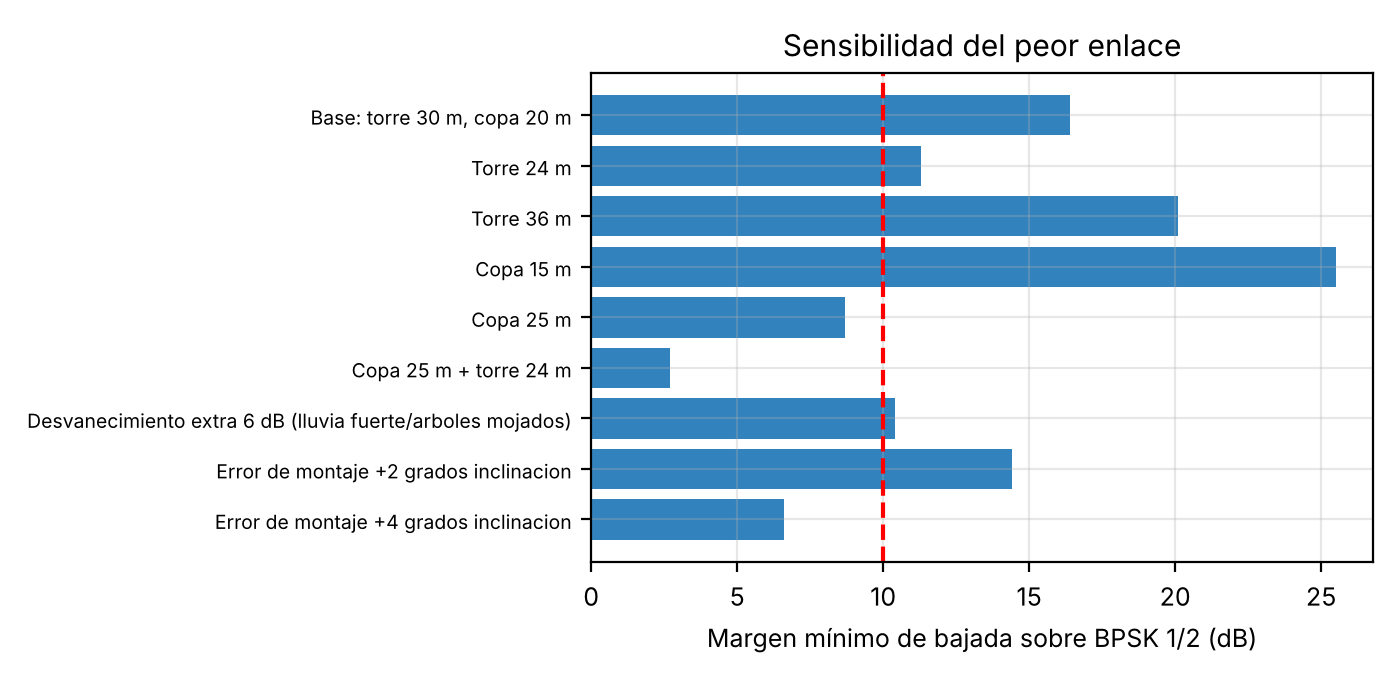
\includegraphics[width=.75\textwidth]{fig_sensibilidad.png}\caption{Margen m\'inimo de bajada por escenario (l\'inea roja: 10\,dB).}\label{fig:sens}\end{figure}
Lectura: el dise\~no base soporta copas hasta $\approx$22\,m y errores de montaje de 2\textdegree{}. Con copas de 25\,m, una casa (la 26) cae bajo 10\,dB y se aplica la contingencia D08. La torre de 24\,m no es suficiente en el peor escenario (copas de 25\,m: margen UL $-0.3$\,dB), lo que confirma la altura de 30\,m.

\section{Energ\'ia, costos y viabilidad}
\subsection{Energ\'ia solar (dimensionamiento breve)}
La energ\'ia no es el foco del proyecto; se dimensiona de forma simple. Carga continua en la torre: Starlink Performance 100\,W (valor alto del rango 75--100\,W \cite{F18,F21}), tres radios de 9.5\,W, router y switch de 15\,W, m\'as 10\,\% de p\'erdidas: 158\,W, es decir 3.8\,kWh/d\'ia. Con 2 d\'ias de autonom\'ia y 90\,\% de profundidad de descarga se requieren 8.4\,kWh: 2 bater\'ias LiFePO$_4$ de 5.12\,kWh (2.4 d\'ias reales) \cite{F29}. Con 3.5 horas solar pico en el mes m\'as desfavorable (supuesto) y rendimiento 0.75, se requieren 1.44\,kWp: 3 paneles de 550\,W \cite{F30}. Con esto, la torre es autosustentable sin red el\'ectrica.
\subsection{CAPEX}
\begin{table}[H]\centering\caption{Lista de materiales y CAPEX (Q; tipo de cambio 7.6445\,GTQ/US\$ \cite{F22}). ``Fuente'' = precio publicado; ``Estim.'' = estimaci\'on por cotizar.}\small\begin{longtable}{p{5.2cm}rrrrr}\toprule Ítem & Cant. & P.\,unit. (Q) & Total (Q) & Estado\\\midrule\endhead
Starlink Performance (Gen 3)\, plato & 1 & 11\,459 & 11\,459 & Fuente\\
Adaptador de tubo Starlink & 1 & 480 & 480 & Fuente\\
Cable Starlink Performance 50 m & 1 & 1\,300 & 1\,300 & Fuente\\
Radio Rocket Prism 5AC Gen2 & 3 & 2\,353 & 7\,058 & Fuente\\
Antena sectorial AM-5G16-120 & 3 & 604 & 1\,812 & Fuente\\
Router PoE + switch central & 1 & 1\,911 & 1\,911 & Estim.\\
Inyectores PoE 24 V para radios & 3 & 191 & 573 & Estim.\\
CPE LiteBeam 5AC Gen2 & 109 & 496 & 54\,020 & Fuente\\
Mástil galvanizado 6 m para CPE & 109 & 191 & 20\,831 & Estim.\\
Cable UTP exterior 15 m + conectores & 109 & 92 & 9\,999 & Estim.\\
Router Wi-Fi interior & 109 & 229 & 24\,998 & Estim.\\
Punto de acceso comunitario exterior & 2 & 1\,368 & 2\,737 & Estim.\\
Torre ventada 30 m (obra civil\, vientos\, pararrayos) & 1 & 57\,334 & 57\,334 & Estim.\\
Puesta a tierra y protección contra descargas & 1 & 6\,116 & 6\,116 & Estim.\\
Cable UTP blindado y accesorios de torre & 1 & 1\,911 & 1\,911 & Estim.\\
Panel solar 550 W & 3 & 1\,261 & 3\,784 & Estim.\\
Batería LiFePO4 48 V 100 Ah (5.12 kWh) & 2 & 26\,725 & 53\,450 & Fuente\\
Controlador MPPT + inversor 1 kW & 1 & 7\,262 & 7\,262 & Estim.\\
Estructura de paneles\, protecciones y gabinete & 1 & 9\,938 & 9\,938 & Estim.\\
Instalación de torre y radios (cuadrilla) & 1 & 22\,934 & 22\,934 & Estim.\\
Instalación de CPE en casas (mano de obra) & 109 & 153 & 16\,665 & Estim.\\
Transporte y viáticos & 1 & 11\,467 & 11\,467 & Estim.\\
\midrule \textbf{Subtotal ítems} & & & \textbf{328\,037} & \\
\midrule \textbf{Flete y aduana} & & & \textbf{32\,804} & \\
\midrule \textbf{Imprevistos} & & & \textbf{36\,084} & \\
\midrule \textbf{CAPEX TOTAL (Q)} & & & \textbf{396\,925} & \\
\midrule \textbf{CAPEX por hogar (Q)} & & & \textbf{4\,050} & \\
\bottomrule\end{longtable}
\end{table}
El CAPEX de dise\~no (109 puntos equipados) es $\approx$Q397\,mil ($\approx$US\$51.9\,mil) incluyendo 10\,\% de flete y aduana y 10\,\% de imprevistos; el IVA se considera acreditable para la empresa operadora. El \textbf{CAPEX por hogar} es Q4{,}050 (dividido entre los 98 hogares del a\~no 3) o Q5{,}156 en el a\~no 1 (65 hogares). La mayor parte son los CPE y la instalaci\'on (abonados), seguida por la torre y la energ\'ia (Fig.~\ref{fig:costos}).
\begin{figure}[H]\centering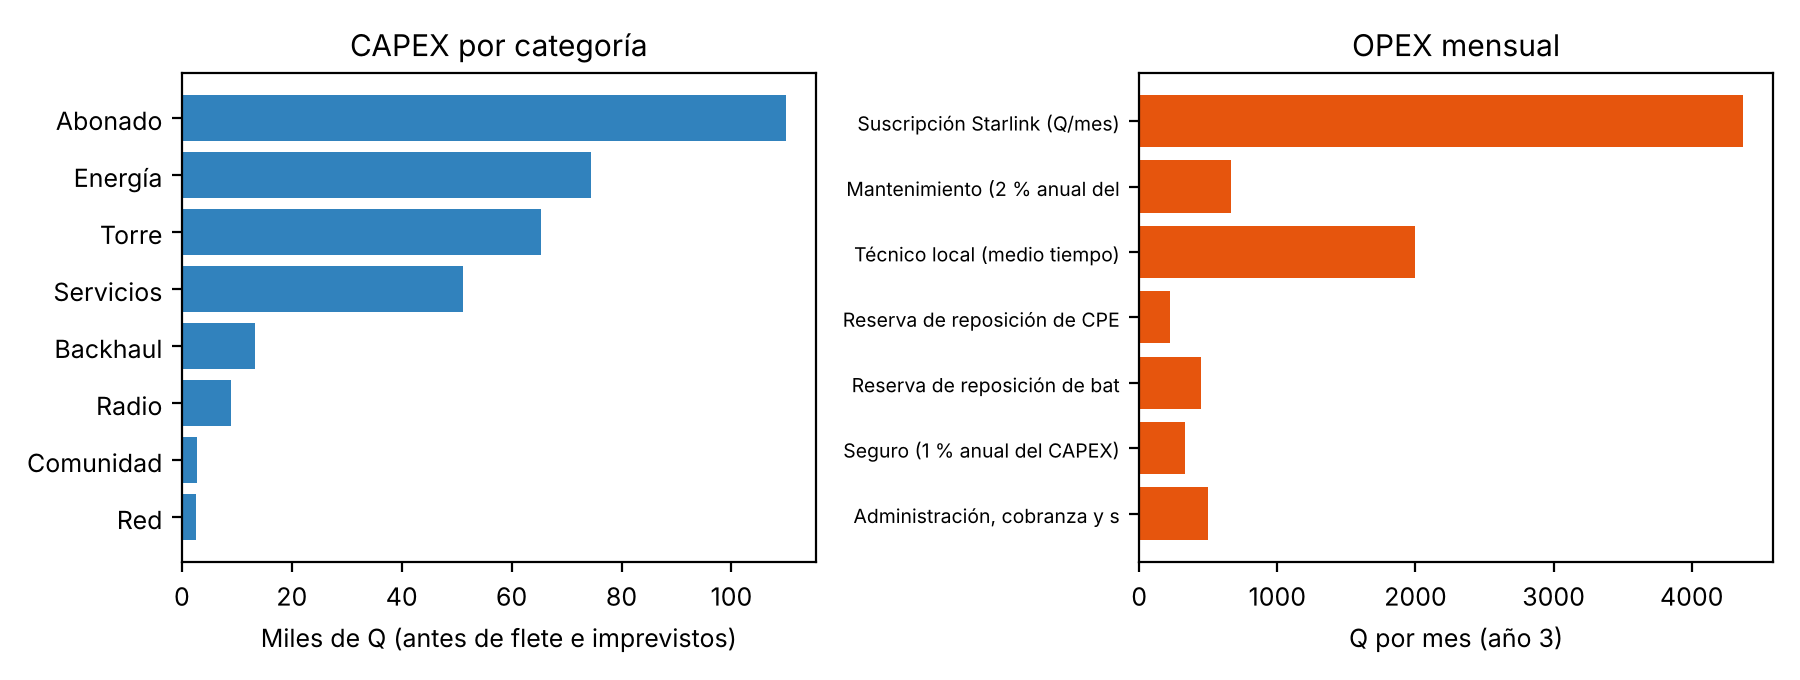
\includegraphics[width=\textwidth]{fig_costos.png}\caption{CAPEX por categor\'ia y OPEX mensual del a\~no 3.}\label{fig:costos}\end{figure}
\subsection{OPEX y tarifa}
\begin{table}[H]\centering\caption{OPEX mensual (Q). Suscripci\'on Starlink: Prioridad Local 2\,TB Q2{,}970 m\'as bloques de 50\,GB a Q140 \cite{F08}.}\small\begin{tabular}{lrr}\toprule Concepto (Q/mes) & Año 1 & Año 3\\\midrule
Suscripción Starlink (Q/mes) & 2\,970 & 4\,370\\
Mantenimiento (2 \% anual del CAPEX) & 559 & 662\\
Técnico local (medio tiempo) & 2\,000 & 2\,000\\
Reserva de reposición de CPE (5 \% anual) & 134 & 225\\
Reserva de reposición de baterías (vida 10 años) & 445 & 445\\
Seguro (1 \% anual del CAPEX) & 279 & 331\\
Administración\, cobranza y soporte & 500 & 500\\
\midrule OPEX MENSUAL TOTAL (Q) & 6\,887 & 8\,533\\
Hogares con servicio & 65 & 98\\
OPEX por hogar por mes (Q) & 106.0 & 87.1\\
Amortización del CAPEX a 5 años por hogar y mes (Q) & 85.9 & 67.5\\
\midrule TARIFA DE EQUILIBRIO por hogar y mes (Q) & 191.9 & 154.6\\
\bottomrule\end{tabular}
\end{table}
En el a\~no 3 el consumo ser\'ia de 2.5\,TB (100 puntos x 25\,GB) y se necesitan 10 bloques extra. El OPEX por hogar es Q87 al mes (a\~no 3) y Q106 (a\~no 1). A\~nadiendo la amortizaci\'on del CAPEX a 5 a\~nos (Q67.5 por hogar y mes), la \textbf{tarifa de equilibrio} es $\approx$Q155 por hogar y mes en el a\~no 3 y Q192 en el a\~no 1. Se propone una tarifa de Q175 mensuales, con la que el CAPEX se recupera en $\approx$46 meses y el servicio es sostenible. Para la alternativa de vender el servicio a menor precio se requerir\'ia un subsidio o un proyecto social.

\section{Marco legal y regulatorio}\label{sec:legal}
Se asume que el proyecto lo ejecuta una empresa operadora ya legalizada. La Ley General de Telecomunicaciones (Decreto 94-96) y su reglamento (Acuerdo Gubernativo 574-98) fijan que la SIT administra el espectro y la Tabla Nacional de Atribuci\'on de Frecuencias (TNAF) \cite{F05,F06}. Los servicios se inscriben en el registro de telecomunicaciones (ORC) \cite{F04}; operar sin t\'itulo o fuera de la banda se sanciona (art.~81, por verificar en el texto oficial). Starlink fue autorizado por la SIT en mayo de 2023 \cite{F02}, por lo que el backhaul se contrata como servicio comercial (Prioridad Local). La referencia regional lista 5725--5850\,MHz entre las bandas de 5\,GHz de Guatemala \cite{F28}; los tres canales del plan (5745, 5785 y 5825\,MHz de 20\,MHz) quedan dentro, con equipos certificados FCC/CE y potencia dentro del l\'imite aplicable, \textbf{por confirmar en la TNAF vigente} (no se pudo acceder al texto oficial desde el entorno de trabajo). Adem\'as: acuerdo con la comunidad (COCODE) para el terreno de la torre; permiso municipal de Chisec para la obra civil; dise\~no de cimentaci\'on, vientos y pararrayos por un profesional; y consideraci\'on de se\~nalizaci\'on a\'erea si aplica. Para el an\'alisis acad\'emico se asume que los derechos de uso del espectro est\'an disponibles.

\section{Riesgos y limitaciones}
\begin{itemize}[nosep]
\item \textbf{Georreferenciaci\'on:} $\pm10$\,m en las casas; la imagen puede estar desactualizada o haber casas ocultas.
\item \textbf{Vegetaci\'on:} la altura de copa (20\,m) y la m\'ascara por color son supuestos; el follaje mojado puede aumentar la p\'erdida (escenario +6\,dB).
\item \textbf{Patrones:} F/B y l\'obulos laterales no figuran en las fichas; se usan modelos calibrados y un tope de 25\,dB. Las sensibilidades de ficha son $\pm2$\,dB.
\item \textbf{Starlink:} el precio del plato es de planificaci\'on (US\$1{,}499) y puede variar; la disponibilidad se verific\'o el 23-oct-2026.
\item \textbf{Precios locales:} los \'items marcados ``Estim.'' deben cotizarse en Guatemala.
\item \textbf{Punto \'unico de falla:} la torre y el plato Starlink; se mitiga con repuestos y autonom\'ia.
\end{itemize}

\section{Conclusiones}
Una sola torre de 30\,m con tres sectores de 5\,GHz y backhaul Starlink conecta las 109 casas de Babilonia con margen de al menos 13.4\,dB sobre BPSK en el peor enlace de subida, a un CAPEX de $\approx$Q4{,}050 por hogar y una tarifa de equilibrio de $\approx$Q155 al mes. El relieve de la hondonada es favorable; la vegetaci\'on determina la altura de la torre y el presupuesto de enlace. El plan de tres canales con sincron\'ia GPS es necesario para evitar interferencia entre sectores. El sistema es robusto frente a variaciones razonables (copas hasta 22\,m, errores de montaje de 2\textdegree) y tiene margen de crecimiento hasta 6\,Mbps de pico por usuario activo.

\section{Organizaci\'on del equipo}\label{sec:equipo}
\begin{table}[H]\centering\begin{tabular}{p{3.8cm}p{9.8cm}}\toprule Integrante & Responsabilidades\\\midrule Kevin Gabriel Gonz\'alez Donis & Selecci\'on de la aldea, arquitectura, presupuesto de enlace, simulaci\'on y libro de c\'alculo\\ Maximiliano Gonz\'alez De Le\'on & Terreno, propagaci\'on y vegetaci\'on, capacidad e interferencia, energ\'ia\\ Diego Andre Cuellar Butcher & Costos y viabilidad, marco legal (SIT), informe y defensa\\\bottomrule\end{tabular}\end{table}

\appendix
\section{Resultados completos por casa}
\small\begin{longtable}{rlrrrrrrl}\toprule Casa & Sec. & Dist. (m) & Elev. rayo (°) & Follaje (m) & Follaje (dB) & Margen DL & Margen UL & MCS DL\\\midrule\endhead
1 & S2 & 297 & 2.7 & 31 & 16.5 & 41.8 & 38.8 & 256QAM 3/4\\
2 & S2 & 233 & 5.1 & 42 & 19.7 & 39.9 & 36.9 & 64QAM 5/6\\
3 & S2 & 201 & 6.2 & 81 & 29.0 & 30.0 & 27.0 & 64QAM 2/3\\
4 & S1 & 190 & 6.4 & 55 & 23.1 & 35.4 & 32.4 & 64QAM 5/6\\
5 & S2 & 209 & 6.6 & 85 & 29.9 & 30.4 & 27.4 & 64QAM 3/4\\
6 & S2 & 185 & 7.6 & 82 & 29.2 & 31.1 & 28.1 & 64QAM 3/4\\
7 & S2 & 217 & 6.2 & 58 & 23.9 & 37.4 & 34.4 & 64QAM 5/6\\
8 & S2 & 269 & 4.0 & 65 & 25.5 & 35.5 & 32.5 & 64QAM 5/6\\
9 & S2 & 295 & 2.9 & 50 & 21.9 & 38.0 & 35.0 & 64QAM 5/6\\
10 & S2 & 287 & 3.4 & 69 & 26.4 & 34.0 & 31.0 & 64QAM 5/6\\
11 & S2 & 322 & 2.3 & 32 & 16.8 & 42.1 & 39.1 & 256QAM 3/4\\
12 & S2 & 314 & 2.8 & 54 & 22.9 & 36.7 & 33.7 & 64QAM 5/6\\
13 & S2 & 171 & 8.4 & 42 & 19.7 & 40.3 & 37.3 & 64QAM 5/6\\
14 & S2 & 164 & 8.8 & 11 & 8.2 & 51.4 & 48.4 & 256QAM 5/6\\
15 & S2 & 164 & 8.8 & 0 & 0.0 & 59.8 & 56.8 & 256QAM 5/6\\
16 & S2 & 132 & 10.8 & 9 & 6.7 & 45.8 & 42.8 & 256QAM 3/4\\
17 & S2 & 76 & 18.2 & 5 & 3.7 & 50.4 & 47.4 & 256QAM 5/6\\
18 & S2 & 161 & 8.6 & 46 & 20.8 & 39.5 & 36.5 & 64QAM 5/6\\
19 & S2 & 195 & 7.1 & 39 & 18.9 & 42.9 & 39.9 & 256QAM 3/4\\
20 & S2 & 259 & 4.9 & 38 & 18.6 & 42.7 & 39.7 & 256QAM 3/4\\
21 & S2 & 288 & 4.2 & 21 & 13.1 & 47.5 & 44.5 & 256QAM 5/6\\
22 & S2 & 323 & 3.5 & 7 & 5.2 & 54.4 & 51.4 & 256QAM 5/6\\
23 & S2 & 374 & 2.9 & 35 & 17.7 & 40.2 & 37.2 & 64QAM 5/6\\
24 & S2 & 394 & 3.0 & 75 & 27.7 & 30.0 & 27.0 & 64QAM 3/4\\
25 & S2 & 420 & 2.8 & 14 & 10.4 & 46.7 & 43.7 & 256QAM 3/4\\
26 & S2 & 398 & 2.8 & 147 & 41.2 & 16.4 & 13.4 & 16QAM 1/2\\
27 & S2 & 376 & 2.2 & 122 & 36.9 & 20.8 & 17.8 & 16QAM 3/4\\
28 & S2 & 281 & 4.1 & 10 & 7.4 & 53.3 & 50.3 & 256QAM 5/6\\
29 & S2 & 302 & 3.4 & 66 & 25.7 & 34.1 & 31.1 & 64QAM 5/6\\
30 & S2 & 328 & 3.0 & 86 & 30.1 & 28.9 & 25.9 & 64QAM 2/3\\
31 & S2 & 337 & 2.6 & 45 & 20.5 & 37.7 & 34.7 & 64QAM 5/6\\
32 & S2 & 307 & 3.0 & 64 & 25.3 & 34.0 & 31.0 & 64QAM 5/6\\
33 & S2 & 267 & 3.6 & 56 & 23.4 & 37.3 & 34.3 & 64QAM 5/6\\
34 & S2 & 234 & 4.0 & 7 & 5.2 & 55.9 & 52.9 & 256QAM 5/6\\
35 & S2 & 198 & 5.5 & 9 & 6.7 & 55.4 & 52.4 & 256QAM 5/6\\
36 & S2 & 143 & 9.1 & 0 & 0.0 & 59.5 & 56.5 & 256QAM 5/6\\
37 & S2 & 126 & 10.1 & 0 & 0.0 & 56.1 & 53.1 & 256QAM 5/6\\
38 & S2 & 109 & 11.8 & 0 & 0.0 & 42.9 & 39.9 & 256QAM 3/4\\
39 & S2 & 93 & 14.0 & 0 & 0.0 & 53.6 & 50.6 & 256QAM 5/6\\
40 & S2 & 81 & 16.5 & 1 & 0.7 & 56.4 & 53.4 & 256QAM 5/6\\
41 & S3 & 81 & 15.3 & 0 & 0.0 & 55.0 & 52.0 & 256QAM 5/6\\
42 & S3 & 60 & 21.0 & 0 & 0.0 & 45.7 & 42.7 & 256QAM 3/4\\
43 & S3 & 50 & 24.4 & 0 & 0.0 & 57.0 & 54.0 & 256QAM 5/6\\
44 & S3 & 89 & 13.5 & 3 & 2.2 & 51.0 & 48.0 & 256QAM 5/6\\
45 & S3 & 109 & 10.8 & 0 & 0.0 & 53.8 & 50.8 & 256QAM 5/6\\
46 & S3 & 112 & 10.3 & 0 & 0.0 & 57.1 & 54.1 & 256QAM 5/6\\
47 & S3 & 104 & 11.3 & 0 & 0.0 & 50.0 & 47.0 & 256QAM 5/6\\
48 & S3 & 90 & 13.1 & 0 & 0.0 & 51.4 & 48.4 & 256QAM 5/6\\
49 & S3 & 93 & 12.4 & 0 & 0.0 & 45.1 & 42.1 & 256QAM 3/4\\
50 & S3 & 71 & 16.6 & 0 & 0.0 & 55.5 & 52.5 & 256QAM 5/6\\
51 & S3 & 90 & 12.5 & 0 & 0.0 & 42.0 & 39.0 & 256QAM 3/4\\
52 & S3 & 104 & 10.3 & 0 & 0.0 & 56.4 & 53.4 & 256QAM 5/6\\
53 & S3 & 110 & 9.9 & 11 & 8.2 & 50.3 & 47.3 & 256QAM 5/6\\
54 & S3 & 120 & 9.0 & 0 & 0.0 & 61.6 & 58.6 & 256QAM 5/6\\
55 & S3 & 165 & 6.3 & 10 & 7.4 & 56.7 & 53.7 & 256QAM 5/6\\
56 & S3 & 140 & 7.2 & 10 & 7.4 & 56.2 & 53.2 & 256QAM 5/6\\
57 & S3 & 118 & 8.8 & 0 & 0.0 & 58.7 & 55.7 & 256QAM 5/6\\
58 & S1 & 125 & 8.4 & 17 & 11.6 & 47.3 & 44.3 & 256QAM 5/6\\
59 & S1 & 87 & 14.2 & 7 & 5.2 & 48.9 & 45.9 & 256QAM 5/6\\
60 & S1 & 122 & 9.4 & 18 & 12.0 & 46.2 & 43.2 & 256QAM 3/4\\
61 & S1 & 135 & 8.5 & 26 & 14.9 & 46.2 & 43.2 & 256QAM 3/4\\
62 & S1 & 104 & 12.1 & 6 & 4.4 & 39.6 & 36.6 & 64QAM 5/6\\
63 & S1 & 124 & 9.6 & 10 & 7.4 & 51.8 & 48.8 & 256QAM 5/6\\
64 & S1 & 68 & 19.4 & 0 & 0.0 & 47.7 & 44.7 & 256QAM 5/6\\
65 & S1 & 101 & 12.7 & 7 & 5.2 & 40.6 & 37.6 & 64QAM 5/6\\
66 & S1 & 103 & 12.4 & 18 & 12.0 & 32.3 & 29.3 & 64QAM 3/4\\
67 & S1 & 104 & 12.1 & 38 & 18.6 & 25.8 & 22.8 & 64QAM 2/3\\
68 & S1 & 138 & 8.5 & 18 & 12.0 & 49.8 & 46.8 & 256QAM 5/6\\
69 & S1 & 128 & 9.3 & 36 & 18.0 & 42.4 & 39.4 & 256QAM 3/4\\
70 & S1 & 137 & 8.9 & 7 & 5.2 & 54.4 & 51.4 & 256QAM 5/6\\
71 & S1 & 116 & 11.3 & 13 & 9.6 & 37.2 & 34.2 & 64QAM 5/6\\
72 & S1 & 82 & 16.4 & 7 & 5.2 & 49.1 & 46.1 & 256QAM 5/6\\
73 & S3 & 142 & 6.8 & 0 & 0.0 & 62.2 & 59.2 & 256QAM 5/6\\
74 & S3 & 154 & 6.3 & 0 & 0.0 & 63.2 & 60.2 & 256QAM 5/6\\
75 & S3 & 187 & 5.0 & 23 & 13.8 & 49.0 & 46.0 & 256QAM 5/6\\
76 & S3 & 204 & 4.5 & 12 & 8.9 & 52.7 & 49.7 & 256QAM 5/6\\
77 & S3 & 158 & 6.1 & 15 & 10.8 & 49.7 & 46.7 & 256QAM 5/6\\
78 & S1 & 172 & 6.0 & 20 & 12.8 & 49.0 & 46.0 & 256QAM 5/6\\
79 & S1 & 178 & 5.8 & 13 & 9.6 & 52.9 & 49.9 & 256QAM 5/6\\
80 & S1 & 189 & 5.1 & 17 & 11.6 & 48.0 & 45.0 & 256QAM 5/6\\
81 & S1 & 196 & 5.1 & 20 & 12.8 & 48.2 & 45.2 & 256QAM 5/6\\
82 & S1 & 208 & 4.7 & 15 & 10.8 & 48.1 & 45.1 & 256QAM 5/6\\
83 & S3 & 224 & 4.5 & 14 & 10.4 & 48.0 & 45.0 & 256QAM 5/6\\
84 & S1 & 241 & 4.3 & 15 & 10.8 & 46.9 & 43.9 & 256QAM 3/4\\
85 & S3 & 256 & 3.4 & 48 & 21.3 & 37.7 & 34.7 & 64QAM 5/6\\
86 & S3 & 319 & 1.3 & 75 & 27.7 & 28.3 & 25.3 & 64QAM 2/3\\
87 & S3 & 344 & 0.6 & 26 & 14.9 & 39.2 & 36.2 & 64QAM 5/6\\
88 & S3 & 300 & 2.1 & 39 & 18.9 & 38.2 & 35.2 & 64QAM 5/6\\
89 & S3 & 290 & 2.6 & 35 & 17.7 & 39.7 & 36.7 & 64QAM 5/6\\
90 & S3 & 281 & 3.4 & 25 & 14.5 & 42.5 & 39.5 & 256QAM 3/4\\
91 & S3 & 331 & 1.9 & 34 & 17.4 & 37.3 & 34.3 & 64QAM 5/6\\
92 & S3 & 373 & 0.2 & 31 & 16.5 & 34.6 & 31.6 & 64QAM 5/6\\
93 & S3 & 402 & -1.0 & 13 & 9.6 & 37.8 & 34.8 & 64QAM 5/6\\
94 & S1 & 272 & 3.9 & 16 & 11.2 & 45.6 & 42.6 & 256QAM 3/4\\
95 & S1 & 324 & 2.6 & 27 & 15.2 & 39.6 & 36.6 & 64QAM 5/6\\
96 & S1 & 347 & 1.9 & 49 & 21.6 & 32.4 & 29.4 & 64QAM 3/4\\
97 & S1 & 269 & 3.9 & 92 & 31.3 & 26.6 & 23.6 & 64QAM 2/3\\
98 & S1 & 274 & 3.6 & 34 & 17.4 & 40.8 & 37.8 & 64QAM 5/6\\
99 & S1 & 246 & 4.1 & 31 & 16.5 & 42.7 & 39.7 & 256QAM 3/4\\
100 & S1 & 227 & 4.4 & 27 & 15.2 & 44.7 & 41.7 & 256QAM 3/4\\
101 & S1 & 238 & 3.9 & 27 & 15.2 & 45.1 & 42.1 & 256QAM 3/4\\
102 & S1 & 222 & 4.2 & 18 & 12.0 & 49.1 & 46.1 & 256QAM 5/6\\
103 & S1 & 267 & 2.3 & 60 & 24.3 & 35.2 & 32.2 & 64QAM 5/6\\
104 & S1 & 318 & 2.9 & 79 & 28.6 & 27.9 & 24.9 & 64QAM 2/3\\
105 & S1 & 353 & 1.7 & 73 & 27.3 & 27.3 & 24.3 & 64QAM 2/3\\
106 & S1 & 359 & 1.0 & 14 & 10.4 & 43.6 & 40.6 & 256QAM 3/4\\
107 & S1 & 355 & 0.5 & 78 & 28.4 & 25.3 & 22.3 & 64QAM 2/3\\
108 & S1 & 385 & 0.0 & 0 & 0.0 & 51.3 & 48.3 & 256QAM 5/6\\
109 & S1 & 405 & -0.9 & 0 & 0.0 & 48.5 & 45.5 & 256QAM 5/6\\
\bottomrule\end{longtable}
\normalsize
\section{Fuentes}
\small\begin{longtable}{p{.9cm}p{5.6cm}p{6.2cm}}\toprule ID & Dato & Fuente\\\midrule\endhead
F01 & Planes Starlink GT: Lite Q365, Max Q545, Roam 100GB Q410, Roam Ilimitado Q820 & \url{https://livinginguatemala.com/digital-nomad/starlink-in-guatemala/}\\
F02 & Lanzamiento 14-jul-2023; SIT autorizó 19-may-2023 & \url{https://www.revistaeyn.com/tecnologia-cultura-digital/starlink-llega-a-guatemala-con-precios-especiales-DC14436342}\\
F03 & Alza de precios Starlink 2026 (EE. UU.) & \url{https://www.satelliteinternet.com/resources/starlink-2026-price-increase/}\\
F04 & Requisitos servicios satelitales (licencia, usuario de facilidades, registro ORC) & \url{https://www.bloomberglinea.com/2022/11/16/starlink-de-elon-musk-en-guatemala-que-necesita-para-que-pueda-operar/}\\
F05 & Decreto 94-96, Acuerdo Gubernativo 574-98, art. 81 sanciones & \url{https://livinginguatemala.com/guides/satellite-messengers-guatemala}\\
F06 & TNAF administrada por SIT & \url{https://dplnews.com/?p=270771}\\
F07 & Censo 2018: 29 \% usa Internet (7+ años); brechas departamentales & \url{https://dplnews.com/censo-refleja-brechas-en-el-uso-de-internet/}\\
F08 & Starlink Business GT, Prioridad Local: 50 GB Q310, 500 GB Q870, 1 TB Q1,570, 2 TB Q2,970; +50 GB Q140. Prioridad Global: 50 GB Q1,920, 500 G & Captura propia starlink.com, 23-oct-2026 (`evidencias/starlink\_busines\\
F09 & Disponibilidad "Disponible ahora"; descarga 145–276 Mbps en 15.88908, -90.53177 & Capturas propias starlink.com (`evidencias/starlink\_*\_babilonia.png`)\\
F10 & Ubicación y entorno de Babilonia, Chisec & Capturas Google Maps (`evidencias/maps\_*`)\\
F11 & Starlink en la zona: subida 21–39 Mbps, latencia 22–32 ms & Capturas propias starlink.com (`evidencias/starlink\_subida\_*`, `starli\\
F12 & Elevaciones (m s. n. m.): centro 206, esquinas 215 / 239 / 227 / 247 & Capturas propias Google Earth (`evidencias/elev\_*`)\\
F13 & 109 casas numeradas y vista oblicua & Capturas propias Google Earth (`evidencias/casas\_numeradas\_109.png`, `\\
F14 & Promedio nacional de personas por hogar: 4.5 (2018) & \url{https://www.ces.uvg.edu.gt/censo2018/documentos/infografias.pdf}\\
F15 & Perfiles de elevación Google Earth P1–P6 (casas 25, 93, 55, 5, 109, 31 $\leftrightarrow$ torre): largos 422.2 / 405.9 / 160.0 / 200.9 / 404.8 / 338.2 m; ele & Capturas propias Google Earth (`evidencias/perfil\_P*`); digitalizado e\\
F16 & Precios de accesorios Starlink línea Personal (Standard 4 / 4X) en GTQ & Capturas propias starlink.com/gt/public/shop (`evidencias/starlink\_acc\\
F17 & Modelo de atenuación por follaje de Weissberger: 1.33$\cdot$f\textasciicircum{}0.284$\cdot$d\textasciicircum{}0.588 (14 $<$ d $\leq$ 400 m), 0.45$\cdot$f\textasciicircum{}0.284$\cdot$d (d $\leq$ 14 m) & \url{https://arxiv.org/pdf/2511.11449}\\
F18 & Starlink Performance (Gen 3): 75–100 W medio, 100–240 V, -40 a 60 °C, IP68/IP69K, FOV 140°, 609×396×40 mm, 5.2 kg & \url{https://www.speedcast.com/shop/starlink-performance-gen3-kit/}\\
F19 & Rebaja Performance: US\$1,499 $\rightarrow$ US\$999 (jul-2025, hasta el 7 jul o agotar existencias) & \url{https://www.notebookcheck.org/Starlink-baja-el-precio-del-plato-Performance-en-500-dolares-para-hacer-sitio-al-modelo-de-velocidad-gigabit.1050831.0.html}\\
F20 & Lanzamiento Performance: US\$1,999, $\approx$ 70 W, IP69K, puerto Ethernet para routers de terceros, 470/48 Mbps & \url{https://www.enter.co/?p=573336}\\
F21 & Consumo Starlink: Gen 3 Standard 75–100 W medio, $\approx$ 20 W en reposo; Gen 2 High Performance 110–150 W & \url{https://www.dishytech.com/how-much-power-does-starlink-use/}\\
F22 & Tipo de cambio: 7.6445 GTQ por USD (26-oct-2026) & \url{https://ru.tradingeconomics.com/usdgtq:cur}\\
F23 & Accesorios Starlink línea Empresas Performance (Gen 3) y categorías de la tienda & Capturas propias (`evidencias/starlink\_accesorios\_performance\_gen3.png\\
F24 & Rocket Prism 5AC Gen2: 28 dBm, sensibilidad por MCS, 9.5 W & \url{https://www.netxl.com/ubiquiti/docs/Rocket%20Prism%20AC%20Gen2%20Datasheet.pdf}\\
F25 & AM-5G16-120: 15–16 dBi, 137°/118°, 8° elev., VSWR 1.5, 1.1 kg, US\$79 & \url{https://uk.store.ui.com/uk/en/products/am-5g1}\\
F26 & AM-5G19-120: 18.6–19.1 dBi, 4° elev., 5.9 kg & csd.com.au, 4cabling\\
F27 & LiteBeam 5AC Gen2: 23 dBi, 25 dBm, -96 dBm, 7 W, US\$64.83 & \url{https://store.ui.com}\\
F28 & Bandas 5 GHz de Guatemala según referencia regional: 5150–5250, 5250–5350, 5725–5850 MHz (potencia, EIRP y DFS por verificar en TNAF vigente & \url{https://flyteccomputers.com/blog/5-ghz-frequency-reference-for-latin-america-and-the-caribbean/}\\
F29 & Batería LiFePO4 Relion RB48V100: 51.2 V, 100 Ah, 5.12 kWh, US\$3,495.95 & \url{https://www.solar-electric.com/relion-rb48v100-lithium-ion-battery-48v.html}\\
F30 & Panel solar 550 W, 144 celdas monocristalino (formato estándar); precio US\$165 es estimación & \url{https://a1solarstore.com/solar-panels/550-watt-solar-panels.html?page_id=93}\\
\bottomrule\end{longtable}
\normalsize
\begin{thebibliography}{99}\footnotesize
\bibitem{F02} Revista E\&N, ``Starlink llega a Guatemala con precios especiales'', \url{https://www.revistaeyn.com/tecnologia-cultura-digital/starlink-llega-a-guatemala-con-precios-especiales-DC14436342}
\bibitem{F04} Bloomberg L\'inea, ``Starlink en Guatemala: qu\'e necesita para operar'', \url{https://www.bloomberglinea.com/2022/11/16/starlink-de-elon-musk-en-guatemala-que-necesita-para-que-pueda-operar/}
\bibitem{F05} Living in Guatemala, \textit{Satellite messengers in Guatemala}, \url{https://livinginguatemala.com/guides/satellite-messengers-guatemala}
\bibitem{F06} DPL News, ``Para qu\'e sirve la TNAF'', \url{https://dplnews.com/?p=270771}
\bibitem{F07} DPL News, ``Censo refleja brechas en el uso de internet'', \url{https://dplnews.com/censo-refleja-brechas-en-el-uso-de-internet/}
\bibitem{F08} Captura propia, starlink.com Guatemala, planes Business, 23-oct-2026.
\bibitem{F09} Capturas propias, starlink.com, disponibilidad y velocidades, 23-oct-2026.
\bibitem{F11} Capturas propias, starlink.com, subida y latencia, 25-oct-2026.
\bibitem{F12} Capturas propias, Google Earth, elevaciones, 25-oct-2026.
\bibitem{F13} Capturas propias, Google Earth, 109 casas numeradas, 25-oct-2026.
\bibitem{F14} INE, Censo 2018, infograf\'ias, \url{https://www.ces.uvg.edu.gt/censo2018/documentos/infografias.pdf}
\bibitem{F15} Capturas propias, perfiles de elevaci\'on Google Earth P1--P6, 26-oct-2026.
\bibitem{F17} M.~A.~Weissberger, \textit{An initial critical summary of models for predicting the attenuation of radio waves by trees}, 1982; \url{https://arxiv.org/pdf/2511.11449}
\bibitem{F18} Speedcast, Starlink Performance Gen3, \url{https://www.speedcast.com/shop/starlink-performance-gen3-kit/}
\bibitem{F21} Dishy Tech, \textit{How much power does Starlink use}, \url{https://www.dishytech.com/how-much-power-does-starlink-use/}
\bibitem{F22} Trading Economics, USD/GTQ, \url{https://ru.tradingeconomics.com/usdgtq:cur}
\bibitem{F24} Ubiquiti, Rocket Prism 5AC Gen2 datasheet, \url{https://www.netxl.com/ubiquiti/docs/Rocket\%20Prism\%20AC\%20Gen2\%20Datasheet.pdf}
\bibitem{F25} Ubiquiti Store, AM-5G16-120, \url{https://uk.store.ui.com/uk/en/products/am-5g1}
\bibitem{F26} Ubiquiti AM-5G19-120, ficha de distribuidor (csd.com.au).
\bibitem{F27} Ubiquiti LiteBeam 5AC Gen2, \url{https://store.ui.com}
\bibitem{F28} Flytec, \textit{5 GHz frequency reference for Latin America and the Caribbean}, \url{https://flyteccomputers.com/blog/5-ghz-frequency-reference-for-latin-america-and-the-caribbean/}
\bibitem{F29} Relion RB48V100, \url{https://www.solar-electric.com/relion-rb48v100-lithium-ion-battery-48v.html}
\bibitem{F30} A1 Solar Store, paneles de 550\,W, \url{https://a1solarstore.com/solar-panels/550-watt-solar-panels.html?page_id=93}
\end{thebibliography}
\end{document}
